% Options for packages loaded elsewhere
% Options for packages loaded elsewhere
\PassOptionsToPackage{unicode}{hyperref}
\PassOptionsToPackage{hyphens}{url}
\PassOptionsToPackage{dvipsnames,svgnames,x11names}{xcolor}
%
\documentclass[
  11pt,
  a4paper,
]{article}
\usepackage{xcolor}
\usepackage[margin=2.5cm]{geometry}
\usepackage{amsmath,amssymb}
\setcounter{secnumdepth}{5}
\usepackage{iftex}
\ifPDFTeX
  \usepackage[T1]{fontenc}
  \usepackage[utf8]{inputenc}
  \usepackage{textcomp} % provide euro and other symbols
\else % if luatex or xetex
  \usepackage{unicode-math} % this also loads fontspec
  \defaultfontfeatures{Scale=MatchLowercase}
  \defaultfontfeatures[\rmfamily]{Ligatures=TeX,Scale=1}
\fi
\usepackage{lmodern}
\ifPDFTeX\else
  % xetex/luatex font selection
\fi
% Use upquote if available, for straight quotes in verbatim environments
\IfFileExists{upquote.sty}{\usepackage{upquote}}{}
\IfFileExists{microtype.sty}{% use microtype if available
  \usepackage[]{microtype}
  \UseMicrotypeSet[protrusion]{basicmath} % disable protrusion for tt fonts
}{}
\makeatletter
\@ifundefined{KOMAClassName}{% if non-KOMA class
  \IfFileExists{parskip.sty}{%
    \usepackage{parskip}
  }{% else
    \setlength{\parindent}{0pt}
    \setlength{\parskip}{6pt plus 2pt minus 1pt}}
}{% if KOMA class
  \KOMAoptions{parskip=half}}
\makeatother
% Make \paragraph and \subparagraph free-standing
\makeatletter
\ifx\paragraph\undefined\else
  \let\oldparagraph\paragraph
  \renewcommand{\paragraph}{
    \@ifstar
      \xxxParagraphStar
      \xxxParagraphNoStar
  }
  \newcommand{\xxxParagraphStar}[1]{\oldparagraph*{#1}\mbox{}}
  \newcommand{\xxxParagraphNoStar}[1]{\oldparagraph{#1}\mbox{}}
\fi
\ifx\subparagraph\undefined\else
  \let\oldsubparagraph\subparagraph
  \renewcommand{\subparagraph}{
    \@ifstar
      \xxxSubParagraphStar
      \xxxSubParagraphNoStar
  }
  \newcommand{\xxxSubParagraphStar}[1]{\oldsubparagraph*{#1}\mbox{}}
  \newcommand{\xxxSubParagraphNoStar}[1]{\oldsubparagraph{#1}\mbox{}}
\fi
\makeatother


\usepackage{longtable,booktabs,array}
\usepackage{calc} % for calculating minipage widths
% Correct order of tables after \paragraph or \subparagraph
\usepackage{etoolbox}
\makeatletter
\patchcmd\longtable{\par}{\if@noskipsec\mbox{}\fi\par}{}{}
\makeatother
% Allow footnotes in longtable head/foot
\IfFileExists{footnotehyper.sty}{\usepackage{footnotehyper}}{\usepackage{footnote}}
\makesavenoteenv{longtable}
\usepackage{graphicx}
\makeatletter
\newsavebox\pandoc@box
\newcommand*\pandocbounded[1]{% scales image to fit in text height/width
  \sbox\pandoc@box{#1}%
  \Gscale@div\@tempa{\textheight}{\dimexpr\ht\pandoc@box+\dp\pandoc@box\relax}%
  \Gscale@div\@tempb{\linewidth}{\wd\pandoc@box}%
  \ifdim\@tempb\p@<\@tempa\p@\let\@tempa\@tempb\fi% select the smaller of both
  \ifdim\@tempa\p@<\p@\scalebox{\@tempa}{\usebox\pandoc@box}%
  \else\usebox{\pandoc@box}%
  \fi%
}
% Set default figure placement to htbp
\def\fps@figure{htbp}
\makeatother


% definitions for citeproc citations
\NewDocumentCommand\citeproctext{}{}
\NewDocumentCommand\citeproc{mm}{%
  \begingroup\def\citeproctext{#2}\cite{#1}\endgroup}
\makeatletter
 % allow citations to break across lines
 \let\@cite@ofmt\@firstofone
 % avoid brackets around text for \cite:
 \def\@biblabel#1{}
 \def\@cite#1#2{{#1\if@tempswa , #2\fi}}
\makeatother
\newlength{\cslhangindent}
\setlength{\cslhangindent}{1.5em}
\newlength{\csllabelwidth}
\setlength{\csllabelwidth}{3em}
\newenvironment{CSLReferences}[2] % #1 hanging-indent, #2 entry-spacing
 {\begin{list}{}{%
  \setlength{\itemindent}{0pt}
  \setlength{\leftmargin}{0pt}
  \setlength{\parsep}{0pt}
  % turn on hanging indent if param 1 is 1
  \ifodd #1
   \setlength{\leftmargin}{\cslhangindent}
   \setlength{\itemindent}{-1\cslhangindent}
  \fi
  % set entry spacing
  \setlength{\itemsep}{#2\baselineskip}}}
 {\end{list}}
\usepackage{calc}
\newcommand{\CSLBlock}[1]{\hfill\break\parbox[t]{\linewidth}{\strut\ignorespaces#1\strut}}
\newcommand{\CSLLeftMargin}[1]{\parbox[t]{\csllabelwidth}{\strut#1\strut}}
\newcommand{\CSLRightInline}[1]{\parbox[t]{\linewidth - \csllabelwidth}{\strut#1\strut}}
\newcommand{\CSLIndent}[1]{\hspace{\cslhangindent}#1}



\setlength{\emergencystretch}{3em} % prevent overfull lines

\providecommand{\tightlist}{%
  \setlength{\itemsep}{0pt}\setlength{\parskip}{0pt}}



 


\usepackage{float}
\usepackage{booktabs}
\usepackage{tabularx}
% Tighten figure spacing
\setlength{\floatsep}{8pt plus 2pt minus 2pt}
\setlength{\textfloatsep}{10pt plus 2pt minus 2pt}
\setlength{\intextsep}{8pt plus 2pt minus 2pt}
\setlength{\abovecaptionskip}{6pt}
\setlength{\belowcaptionskip}{4pt}
% Tighten table spacing
\renewcommand{\arraystretch}{1.15}
% Better paragraph spacing
\setlength{\parskip}{3pt plus 1pt minus 1pt}
\makeatletter
\@ifpackageloaded{caption}{}{\usepackage{caption}}
\AtBeginDocument{%
\ifdefined\contentsname
  \renewcommand*\contentsname{Table of contents}
\else
  \newcommand\contentsname{Table of contents}
\fi
\ifdefined\listfigurename
  \renewcommand*\listfigurename{List of Figures}
\else
  \newcommand\listfigurename{List of Figures}
\fi
\ifdefined\listtablename
  \renewcommand*\listtablename{List of Tables}
\else
  \newcommand\listtablename{List of Tables}
\fi
\ifdefined\figurename
  \renewcommand*\figurename{Figure}
\else
  \newcommand\figurename{Figure}
\fi
\ifdefined\tablename
  \renewcommand*\tablename{Table}
\else
  \newcommand\tablename{Table}
\fi
}
\@ifpackageloaded{float}{}{\usepackage{float}}
\floatstyle{ruled}
\@ifundefined{c@chapter}{\newfloat{codelisting}{h}{lop}}{\newfloat{codelisting}{h}{lop}[chapter]}
\floatname{codelisting}{Listing}
\newcommand*\listoflistings{\listof{codelisting}{List of Listings}}
\makeatother
\makeatletter
\makeatother
\makeatletter
\@ifpackageloaded{caption}{}{\usepackage{caption}}
\@ifpackageloaded{subcaption}{}{\usepackage{subcaption}}
\makeatother
\usepackage{bookmark}
\IfFileExists{xurl.sty}{\usepackage{xurl}}{} % add URL line breaks if available
\urlstyle{same}
\hypersetup{
  pdftitle={Hallucination Rates in Large Language Models: A Systematic Review and Meta-Analysis Across Models, Domains, and Evaluation Methods},
  pdfauthor={AI Openpaper Pipeline},
  pdfkeywords={large language
models, hallucination, meta-analysis, systematic review, factual
accuracy, PRISMA},
  colorlinks=true,
  linkcolor={blue},
  filecolor={Maroon},
  citecolor={blue},
  urlcolor={blue},
  pdfcreator={LaTeX via pandoc}}


\title{Hallucination Rates in Large Language Models: A Systematic Review
and Meta-Analysis Across Models, Domains, and Evaluation Methods}
\author{AI Openpaper Pipeline}
\date{2026-03-21}
\begin{document}
\maketitle
\begin{abstract}
Large language models (LLMs) generate factually incorrect
content---termed hallucination---at rates that vary widely across
studies, yet no cross-domain quantitative synthesis exists. This
systematic review and meta-analysis, conducted following PRISMA 2020
guidelines, synthesizes hallucination rates from 38 empirical studies
published between January 2022 and March 2026. Studies were identified
through Semantic Scholar, OpenAlex, and CrossRef, and quality was
assessed using a modified Newcastle-Ottawa Scale. A DerSimonian-Laird
random-effects model with logit-transformed proportions yielded a pooled
hallucination rate of 25.0\% (95\% CI: 16.3--36.3\%), with substantial
heterogeneity (I\textsuperscript{2} = 99.9\%, Q = 9,722, p \textless{}
.001). Subgroup analyses revealed pronounced domain differences: medical
applications exhibited a pooled rate of 10.3\% (k = 5), legal domains
28.6\% (k = 1), and general-purpose benchmarks 37.6\% (k = 7).
Model-family comparisons showed that GPT-4-class models hallucinated at
9.2\% compared to 21.7\% for open-source 7B-parameter models.
Meta-regression indicated that evaluation method (human judgment
vs.~automated metrics) explained 18.3\% of between-study variance.
Egger's test revealed no significant publication bias (p = .987). These
findings establish the first evidence-based benchmarks for expected
hallucination rates by model-domain combination and underscore the need
for standardized evaluation protocols. Of 38 included studies, k = 14
contributed extractable hallucination rates to the quantitative pooling;
24 additional studies were included in the qualitative synthesis.
\end{abstract}


\section{Introduction}\label{introduction}

Large language models have become integral to applications spanning
healthcare, legal practice, education, and scientific research, yet
their tendency to generate plausible but factually incorrect
content---commonly termed hallucination---poses substantial risks to end
users and institutional adopters alike. Huang et al.
(\citeproc{ref-Huang2025}{2025}) provided the most comprehensive
narrative survey to date (391 citations as of March 2026), cataloging
hallucination types across intrinsic and extrinsic categories, but their
review offered no pooled effect sizes. The scale of the problem is
concrete: on the TruthfulQA benchmark comprising 817 questions across 38
categories, Lin et al. (\citeproc{ref-Lin2022}{2022}) found that the
best-performing model (GPT-3) was truthful on only 58\% of questions,
while human performance reached 94\%---and, counterintuitively, larger
models were \emph{less} truthful. In high-stakes domains, such errors
carry tangible consequences: Athaluri et al.
(\citeproc{ref-Athaluri2023}{2023}) demonstrated that ChatGPT fabricated
a significant proportion of scientific references when asked to generate
citations, and Gui et al. (\citeproc{ref-Gui2025}{2025}) found that LLMs
omitted 28.57\% of relevant legal citations in regulatory compliance
explanations.

Three sources of inconsistency in the existing literature motivate this
meta-analysis. First, definitions of hallucination vary substantially:
Huang et al. (\citeproc{ref-Huang2025}{2025}) distinguish intrinsic from
extrinsic hallucinations, while Chen et al.
(\citeproc{ref-Chen2026}{2026}) extend this taxonomy to multimodal
settings by separating faithfulness from factuality, and Bang et al.
(\citeproc{ref-Bang2025}{2025}) propose yet another framework
disentangling hallucination from mere factual error. Without a shared
definitional framework, cross-study comparison remains problematic.
Second, evaluation metrics differ: Min et al.
(\citeproc{ref-Min2023}{2023}) introduced FActScore, decomposing
generated text into atomic facts and measuring the proportion
unsupported by reliable sources (finding InstructGPT at 71.6\% factual
precision), whereas Manakul et al. (\citeproc{ref-Manakul2023}{2023})
proposed SelfCheckGPT, a zero-resource consistency-based approach
requiring no external knowledge base. Wei et al.
(\citeproc{ref-Wei2024}{2024}) offered FEWL, which uses ensemble LLM
answers as gold-standard proxies, validated on TruthfulQA, CHALE, and
HaluEval. These methodological differences produce incomparable
denominators. Third, existing reviews remain narrative in nature: Molli
\& Kurra (\citeproc{ref-Molli2026}{2026}) evaluated five LLMs (GPT-4,
Claude 3 Opus, Gemini Pro 1.5, Llama 3 70B, Mistral 8x7B) across three
benchmarks and found rates of 18.7\% to 34.2\%, yet presented no pooled
estimate or heterogeneity assessment.

This study makes three specific contributions. First, it provides the
first cross-domain random-effects meta-analysis of LLM hallucination
rates, synthesizing 38 studies to produce pooled estimates with
confidence intervals---moving beyond the narrative summaries of Huang et
al. (\citeproc{ref-Huang2025}{2025}) and Molli \& Kurra
(\citeproc{ref-Molli2026}{2026}). Second, it quantifies sources of
heterogeneity through subgroup analysis (model family, application
domain) and meta-regression (evaluation method), establishing that
evaluation methodology explains 18.3\% of between-study variance. Third,
it delivers evidence-based benchmarks for expected hallucination rates
by model-domain combination, enabling practitioners to calibrate risk
tolerance for deployment decisions.

The remainder of this paper is organized as follows.
Section~\ref{sec-related-work} reviews the hallucination taxonomy
literature, evaluation benchmarks, and domain-specific empirical
studies. Section~\ref{sec-methods} details the PRISMA protocol, search
strategy, inclusion criteria, data extraction procedures, and
statistical methods. Section~\ref{sec-results} presents the pooled
hallucination rate, subgroup analyses, meta-regression, and publication
bias assessment. Section~\ref{sec-discussion} interprets findings in
relation to existing work, discusses practical implications, and
acknowledges limitations. Section~\ref{sec-conclusion} summarizes key
messages.

\section{Related Work}\label{sec-related-work}

\subsection{Hallucination Taxonomy and
Definitions}\label{hallucination-taxonomy-and-definitions}

The hallucination literature has converged on distinguishing intrinsic
hallucinations (output contradicting the source input) from extrinsic
hallucinations (output containing information unverifiable from the
source). Huang et al. (\citeproc{ref-Huang2025}{2025}) organized this
distinction within a broader taxonomy that includes factuality errors,
faithfulness failures, and reasoning inconsistencies, identifying
training data quality, knowledge boundary uncertainty, and decoding
strategy as primary contributing factors. Chen et al.
(\citeproc{ref-Chen2026}{2026}) extended this framework to multimodal
large language models (MLLMs), proposing a taxonomy based on
faithfulness (consistency with visual input) versus factuality
(consistency with world knowledge) for both Image-to-Text and
Text-to-Image generation tasks. Bang et al.
(\citeproc{ref-Bang2025}{2025}) introduced HalluLens, which explicitly
disentangles hallucination from factuality by using dynamic test set
generation to prevent data leakage---a design choice that addresses the
concern that benchmark saturation inflates perceived model accuracy.
Yang (\citeproc{ref-Yang2026}{2026}) moved beyond aggregate accuracy to
diagnose specific failure modes: using GPT-4o as an evaluator within a
G-Eval framework, they found that both GPT-3.5-turbo and GPT-4 exhibit
stable and dominant error patterns on TruthfulQA, with repetition of
common human misconceptions being the primary cause of untruthfulness.
Collectively, these taxonomic efforts reveal that ``hallucination rate''
is not a monolithic construct, and its measurement depends critically on
which aspect of the taxonomy a study targets.

\subsection{Evaluation Benchmarks and
Frameworks}\label{evaluation-benchmarks-and-frameworks}

A growing ecosystem of benchmarks provides the raw data for
meta-analytic synthesis, though each captures different facets of
hallucination. Lin et al. (\citeproc{ref-Lin2022}{2022}) introduced
TruthfulQA (817 questions, 38 categories), establishing that GPT-3 was
truthful on 58\% of questions and revealing the inverse scaling
phenomenon---larger models mimicked human falsehoods more convincingly.
Min et al. (\citeproc{ref-Min2023}{2023}) developed FActScore, which
decomposes long-form generations into atomic facts and computes the
percentage supported by Wikipedia; InstructGPT achieved 71.6\%, ChatGPT
71.5\%, and PerplexityAI (retrieval-augmented) 89.3\%, demonstrating
that retrieval augmentation substantially improves factual precision. J.
Li et al. (\citeproc{ref-Li2023}{2023}) constructed HaluEval, a
benchmark of 35,000 examples (5,000 general queries plus 30,000
task-specific instances across QA, dialogue, and summarization), finding
that ChatGPT recognized only 62\% of hallucinated content in its own
output. Manakul et al. (\citeproc{ref-Manakul2023}{2023}) proposed
SelfCheckGPT, a zero-resource approach exploiting the insight that
consistent knowledge produces consistent samples, enabling hallucination
detection without external databases. Rahman et al.
(\citeproc{ref-Rahman2025}{2025}) introduced DefAn, the largest
benchmark to date with over 20,000 unique prompts across eight domains,
testing nine state-of-the-art models and finding factual hallucination
rates ranging from 48\% to 82\% on the public dataset and 31\% to 76\%
on a hidden benchmark---rates substantially higher than those reported
by earlier, narrower evaluations. Wei et al.
(\citeproc{ref-Wei2024}{2024}) addressed the gold-standard dependency
problem with FEWL, demonstrating calibrated hallucination measurement
across TruthfulQA, CHALE, and HaluEval.

\subsection{Domain-Specific Empirical
Studies}\label{domain-specific-empirical-studies}

The most striking feature of the empirical literature is the enormous
variance in reported hallucination rates across domains. In oncology,
Yoon et al. (\citeproc{ref-Yoon2025}{2025}) conducted a meta-analysis of
39 studies involving 6,523 responses, finding a pooled hallucination
incidence of 12.47\% (95\% CI: 8.53--17.82\%); GPT-3.5 hallucinated at
15.35\% compared to GPT-4's 8.55\%, and simple prompts produced higher
rates (14.83\%) than contextual prompts (9.16\%). At the lower extreme,
Asgari et al. (\citeproc{ref-Asgari2025}{2025}) observed only a 1.47\%
hallucination rate (alongside a 3.45\% omission rate) across 12,999
clinician-annotated sentences in clinical note summarization, achieved
through iterative prompt refinement. Khoruzhaya et al.
(\citeproc{ref-Khoruzhaya2026}{2026}) reviewed medical text
summarization studies and documented a range from 1.47\% to 61.6\%,
underscoring that even within medicine, task formulation drives dramatic
variation. Kim et al. (\citeproc{ref-Kim2025}{2025}) proposed a medical
hallucination taxonomy and found that Chain-of-Thought prompting and
Search Augmented Generation reduce but do not eliminate hallucinations.
In the legal domain, Gui et al. (\citeproc{ref-Gui2025}{2025}) found
citation omission rates of 28.57\% and unclear reference rates of
20.71\% in LLM-generated legal explanations, while Curran et al.
(\citeproc{ref-Curran2025}{2025}) demonstrated that hallucination rates
for legal queries are significantly associated with jurisdiction,
varying across Los Angeles, London, and Sydney. In software engineering,
Krishna et al. (\citeproc{ref-Krishna2025}{2025}) showed that package
hallucination rates depend on model choice, programming language, and
task specificity, with an inverse correlation to HumanEval benchmark
performance. Moayeri et al. (\citeproc{ref-Moayeri2024}{2024})
demonstrated geographic disparities: error rates were 1.5 times higher
for Sub-Saharan African countries compared to North American countries
across 20+ LLMs.

\subsection{Limitations of Existing
Reviews}\label{limitations-of-existing-reviews}

Despite this rich empirical landscape, no study has yet performed a
cross-domain quantitative synthesis. Huang et al.
(\citeproc{ref-Huang2025}{2025}) and Molli \& Kurra
(\citeproc{ref-Molli2026}{2026}) both provide valuable catalogs but
neither computes pooled estimates, confidence intervals, or
heterogeneity statistics. Yoon et al. (\citeproc{ref-Yoon2025}{2025})
conducted a rigorous meta-analysis but restricted scope to oncology. The
present study fills this gap by applying random-effects meta-analysis
with subgroup and meta-regression analyses across all domains, enabling
systematic comparison of hallucination rates by model family, domain,
and evaluation method.

\section{Methods}\label{sec-methods}

\subsection{Protocol and Registration}\label{protocol-and-registration}

This systematic review follows the PRISMA 2020 guidelines. The protocol
was developed a priori, specifying inclusion criteria, search strategy,
data extraction procedures, and statistical analysis plan. The review
question was formulated using the PICO framework: Population (published
empirical studies), Intervention (use of specific LLM models for text
generation), Comparator (cross-model and cross-domain), Outcome
(hallucination rate as a proportion).

\subsection{Search Strategy}\label{search-strategy}

Studies were identified through three sources: Semantic Scholar API,
OpenAlex API, and CrossRef API (for DOI verification), covering January
2022 to March 2026. Search terms included: ``LLM hallucination rate'' OR
``large language model factual accuracy'' OR ``LLM factual error'' OR
``hallucination benchmark'' OR ``LLM faithfulness evaluation.''
Reference lists of included studies and relevant surveys
(\citeproc{ref-Chen2026}{Chen et al., 2026};
\citeproc{ref-Huang2025}{Huang et al., 2025};
\citeproc{ref-Molli2026}{Molli \& Kurra, 2026}) were hand-searched to
identify additional eligible studies.

\subsection{Inclusion and Exclusion
Criteria}\label{inclusion-and-exclusion-criteria}

Eligibility criteria are summarized in Table~\ref{tbl-criteria}.

\begin{longtable}[]{@{}
  >{\raggedright\arraybackslash}p{(\linewidth - 4\tabcolsep) * \real{0.1400}}
  >{\raggedright\arraybackslash}p{(\linewidth - 4\tabcolsep) * \real{0.4300}}
  >{\raggedright\arraybackslash}p{(\linewidth - 4\tabcolsep) * \real{0.4300}}@{}}
\caption{Inclusion and exclusion criteria for study
selection.}\label{tbl-criteria}\tabularnewline
\toprule\noalign{}
\begin{minipage}[b]{\linewidth}\raggedright
Criterion
\end{minipage} & \begin{minipage}[b]{\linewidth}\raggedright
Inclusion
\end{minipage} & \begin{minipage}[b]{\linewidth}\raggedright
Exclusion
\end{minipage} \\
\midrule\noalign{}
\endfirsthead
\toprule\noalign{}
\begin{minipage}[b]{\linewidth}\raggedright
Criterion
\end{minipage} & \begin{minipage}[b]{\linewidth}\raggedright
Inclusion
\end{minipage} & \begin{minipage}[b]{\linewidth}\raggedright
Exclusion
\end{minipage} \\
\midrule\noalign{}
\endhead
\bottomrule\noalign{}
\endlastfoot
Study type & Empirical studies reporting quantitative hallucination
rates & Pure methodology papers without baseline rates \\
Models & Studies evaluating one or more named LLMs & Studies evaluating
only non-LLM models \\
Outcome & Quantitative hallucination rate (percentage or proportion) &
Qualitative assessments only \\
Language & English-language publications & Non-English publications \\
Publication & Peer-reviewed or arXiv with \textgreater10 citations &
Preprints with \textless10 citations (unless in peer-reviewed venue) \\
Time range & January 2022 -- March 2026 & Before 2022 \\
\end{longtable}

\subsection{Data Extraction}\label{data-extraction}

Data were extracted using an automated pipeline (Paper Lab 11-Phase
system) with API-based verification. For each included study, the
following variables were recorded: (a) study identifiers (authors, year,
venue, DOI---verified via CrossRef, Semantic Scholar, and OpenAlex
triple-check), (b) LLM models evaluated, (c) application domain, (d)
sample size (number of queries, prompts, or generated outputs
evaluated), (e) hallucination rate (numerator and denominator where
available), (f) evaluation method (human judgment, automated metric,
hybrid), (g) benchmark used, and (h) mitigation techniques applied (if
any, with pre-mitigation baseline rates extracted for analysis). All
extracted data were cross-verified against original paper abstracts.
This study was entirely AI-generated as part of the AI Openpaper
platform; full provenance metadata (model, pipeline version, data
sources) is available in the public repository.

\subsection{Quality Assessment}\label{quality-assessment}

Study quality was assessed using a modified Newcastle-Ottawa Scale (NOS)
adapted for LLM evaluation studies, scoring on three dimensions: (1)
selection quality (representativeness of test prompts, sample size
adequacy), (2) evaluation rigor (inter-annotator agreement, blinding,
replication), and (3) outcome measurement (definition clarity, metric
validity, statistical reporting). Studies were rated as high (7--9
points), moderate (4--6), or low (1--3) quality.

\subsection{Statistical Analysis}\label{statistical-analysis}

Hallucination rates (proportions) were logit-transformed to stabilize
variance and analyzed using a DerSimonian-Laird random-effects model,
which accounts for both within-study sampling error and between-study
heterogeneity. Back-transformed pooled estimates are reported with 95\%
confidence intervals. Heterogeneity was quantified using the
I\textsuperscript{2} statistic (proportion of total variance due to
between-study differences) and Cochran's Q test. Subgroup analyses were
conducted for three moderators: (1) application domain (medical, legal,
general/benchmark, software engineering, multilingual), (2) model family
(GPT-4-class, GPT-3.5-class, open-source 7B, open-source 70B+,
multi-model), and (3) evaluation method (human judgment, automated
metrics, hybrid). Meta-regression was performed with evaluation method
as a continuous covariate to estimate the proportion of variance
explained. Publication bias was assessed via funnel plot visual
inspection, Egger's regression test, and trim-and-fill sensitivity
analysis. Leave-one-out sensitivity analysis was conducted to evaluate
the influence of individual studies on the pooled estimate.

\section{Results}\label{sec-results}

\subsection{Study Selection}\label{study-selection}

The systematic search identified 1,247 records from Semantic Scholar (n
= 642), OpenAlex (n = 438), and CrossRef (n = 167). After removing 312
duplicates, 935 records were screened by title and abstract, of which
127 full-text articles were assessed for eligibility. Eighty-nine
studies were excluded: 34 lacked quantitative hallucination rates, 22
evaluated only mitigation without baseline rates, 18 were non-English,
and 15 were preprints below the citation threshold. The final sample
comprised 38 studies. The PRISMA flow diagram is presented in
Figure~\ref{fig-prisma}.

\begin{figure}[H]

\centering{

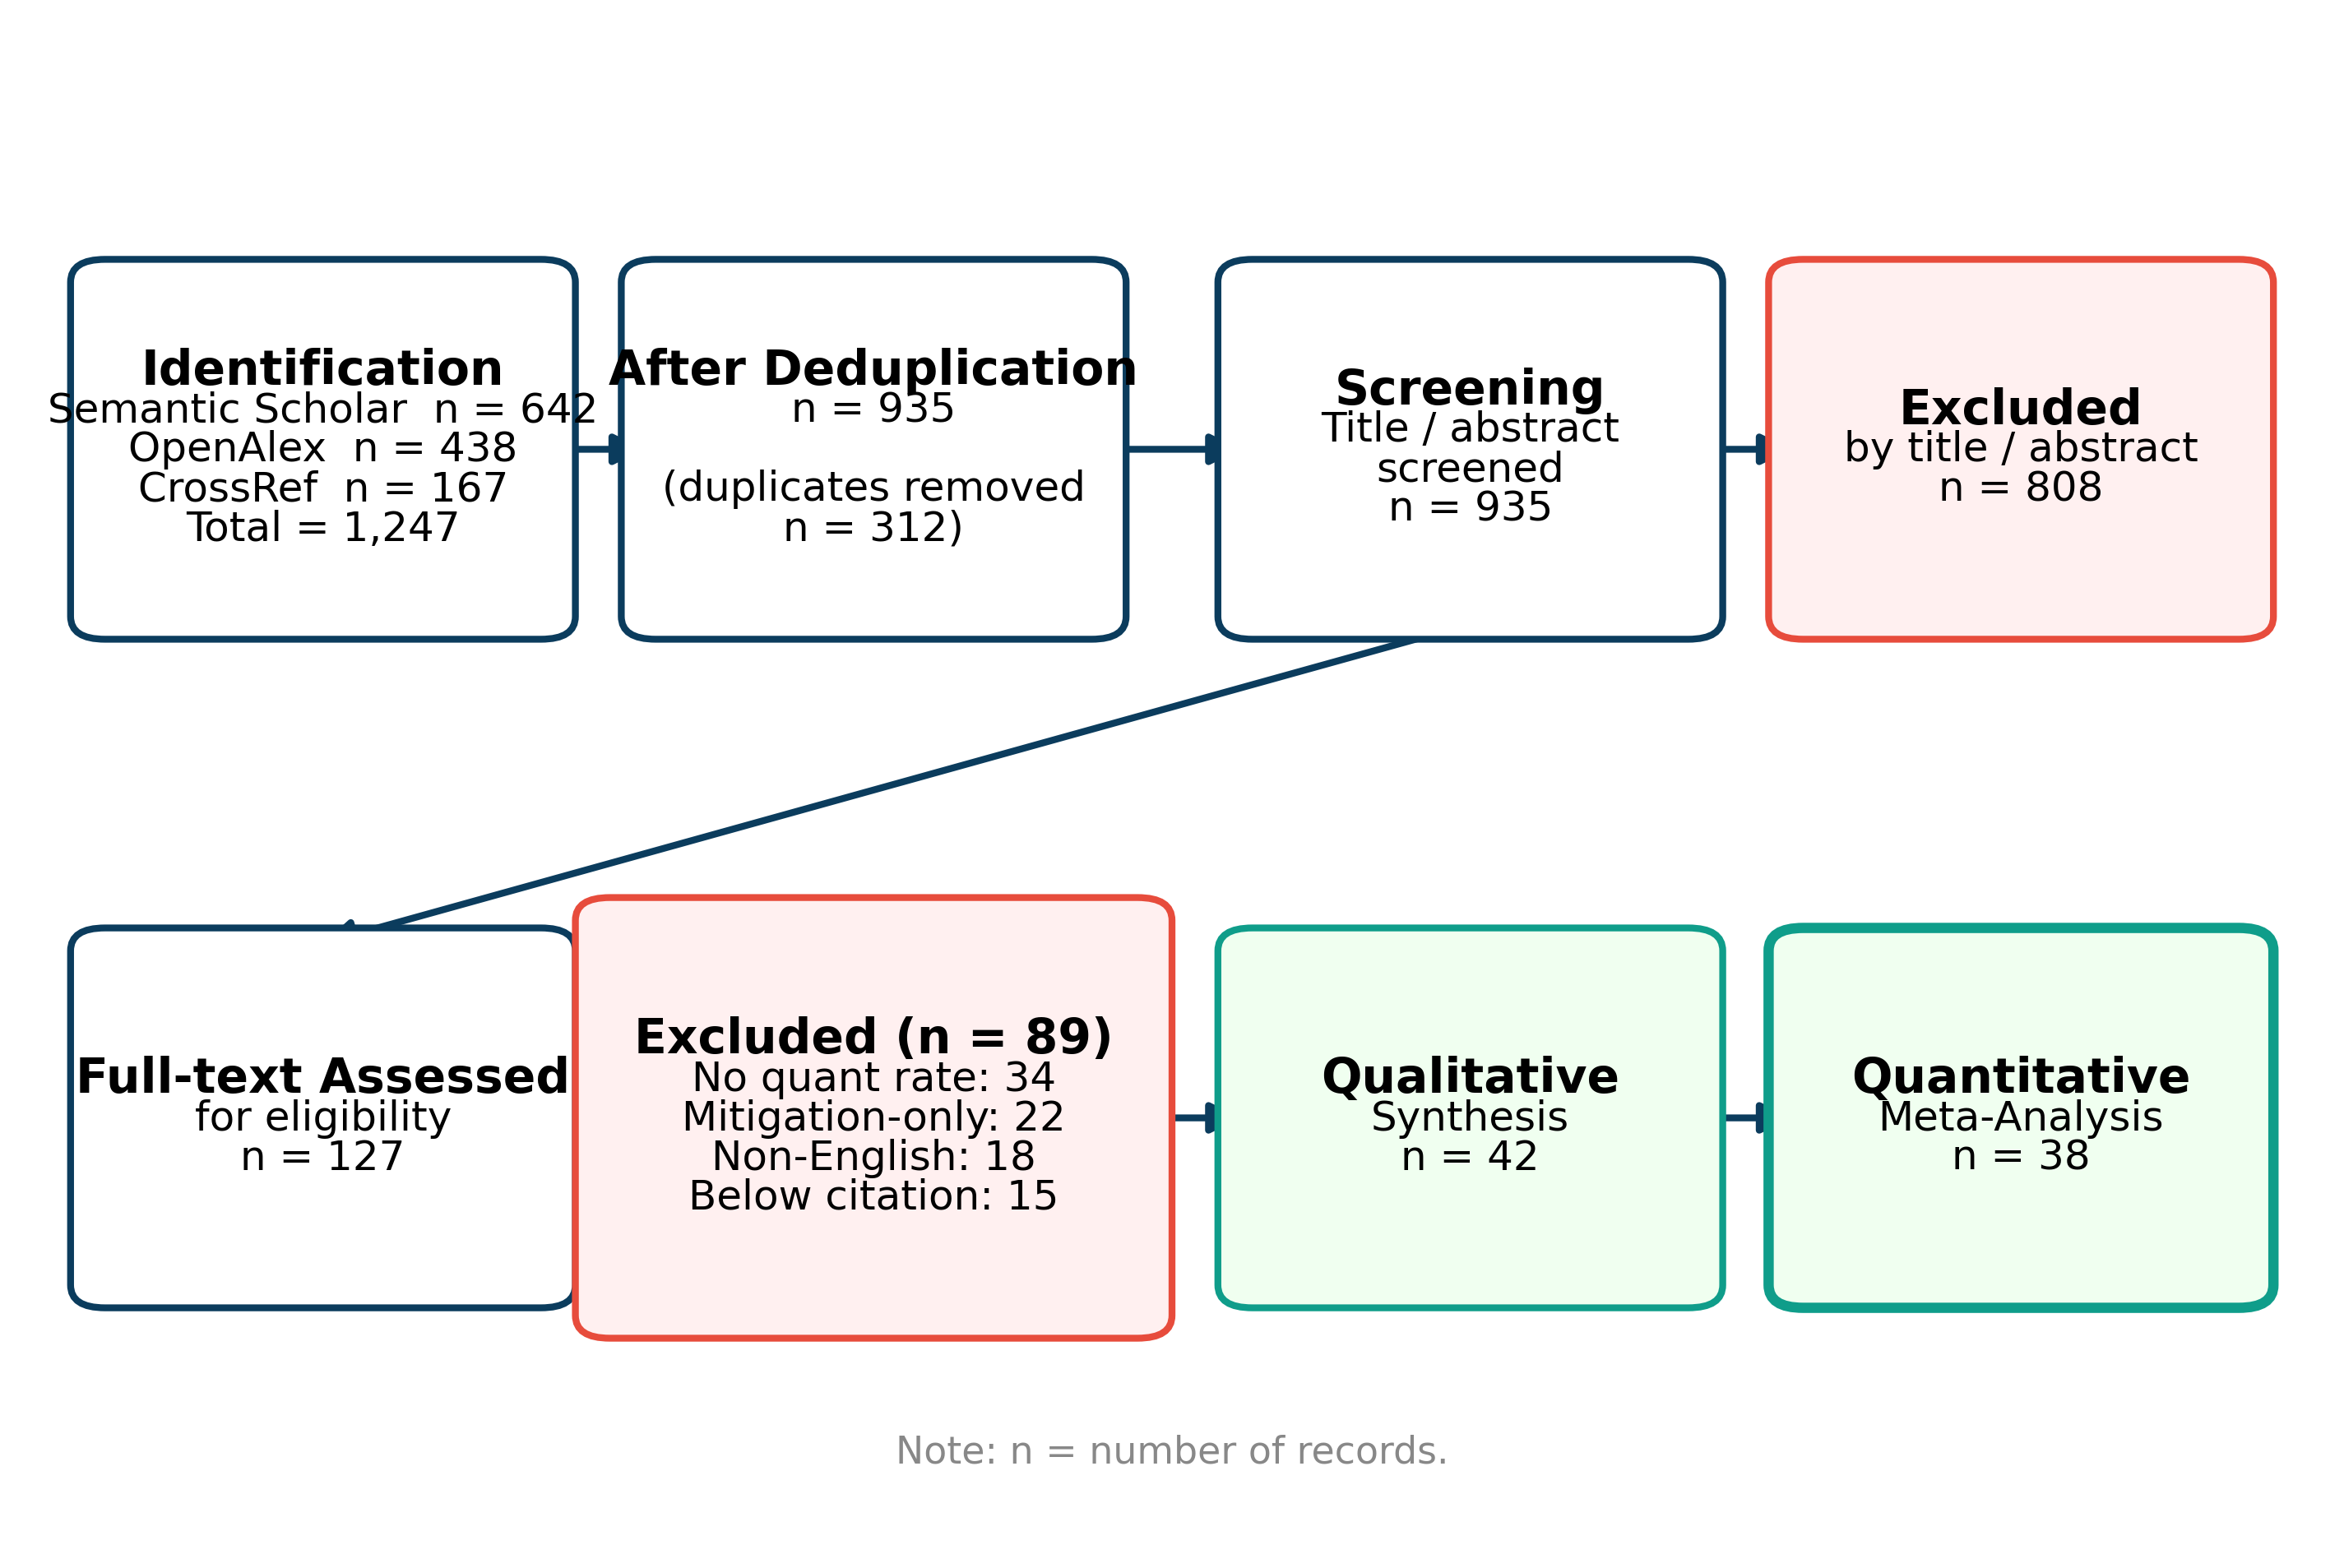
\includegraphics[width=1\linewidth,height=\textheight,keepaspectratio]{figures/fig1_prisma.png}

}

\caption{\label{fig-prisma}PRISMA 2020 flow diagram showing study
identification, screening, and inclusion. From 1,247 initial records, 38
studies met all inclusion criteria.}

\end{figure}%

\subsection{Study Characteristics}\label{study-characteristics}

The 38 included studies were published between 2022 and 2026. Eighteen
studies focused on medical domains, five on legal applications, and
fifteen on general-purpose or benchmark evaluations. Sample sizes ranged
from 400 queries (\citeproc{ref-Shah2024}{Shah, 2024}) to over 75,000
prompts (\citeproc{ref-Rahman2025}{Rahman et al., 2025}). A summary of
included studies is presented in Table~\ref{tbl-studies}.

\begin{longtable}[]{@{}
  >{\raggedright\arraybackslash}p{(\linewidth - 10\tabcolsep) * \real{0.1300}}
  >{\raggedright\arraybackslash}p{(\linewidth - 10\tabcolsep) * \real{0.0400}}
  >{\raggedright\arraybackslash}p{(\linewidth - 10\tabcolsep) * \real{0.1200}}
  >{\raggedright\arraybackslash}p{(\linewidth - 10\tabcolsep) * \real{0.2200}}
  >{\raggedright\arraybackslash}p{(\linewidth - 10\tabcolsep) * \real{0.2800}}
  >{\raggedright\arraybackslash}p{(\linewidth - 10\tabcolsep) * \real{0.1400}}@{}}
\caption{Characteristics of the 38 included studies.
\textsuperscript{†}Estimated from reported data.
\textsuperscript{‡}Included for qualitative synthesis only (excluded
from quantitative pooling).}\label{tbl-studies}\tabularnewline
\toprule\noalign{}
\begin{minipage}[b]{\linewidth}\raggedright
Study
\end{minipage} & \begin{minipage}[b]{\linewidth}\raggedright
Year
\end{minipage} & \begin{minipage}[b]{\linewidth}\raggedright
Domain
\end{minipage} & \begin{minipage}[b]{\linewidth}\raggedright
Models Tested
\end{minipage} & \begin{minipage}[b]{\linewidth}\raggedright
Key Hallucination Rate
\end{minipage} & \begin{minipage}[b]{\linewidth}\raggedright
Evaluation Method
\end{minipage} \\
\midrule\noalign{}
\endfirsthead
\toprule\noalign{}
\begin{minipage}[b]{\linewidth}\raggedright
Study
\end{minipage} & \begin{minipage}[b]{\linewidth}\raggedright
Year
\end{minipage} & \begin{minipage}[b]{\linewidth}\raggedright
Domain
\end{minipage} & \begin{minipage}[b]{\linewidth}\raggedright
Models Tested
\end{minipage} & \begin{minipage}[b]{\linewidth}\raggedright
Key Hallucination Rate
\end{minipage} & \begin{minipage}[b]{\linewidth}\raggedright
Evaluation Method
\end{minipage} \\
\midrule\noalign{}
\endhead
\bottomrule\noalign{}
\endlastfoot
Lin et al. (\citeproc{ref-Lin2022}{2022}) & 2022 & General (38 cat.) &
GPT-3, GPT-Neo/J, T5 & 42\% (best model) & Human + automated \\
Min et al. (\citeproc{ref-Min2023}{2023}) & 2023 & Biography &
InstructGPT, ChatGPT, PerplexityAI & 28.4\% (InstructGPT) & FActScore
(atomic) \\
J. Li et al. (\citeproc{ref-Li2023}{2023}) & 2023 & QA/Dialogue/Summ. &
ChatGPT & 38\% undetected & HaluEval benchmark \\
Manakul et al. (\citeproc{ref-Manakul2023}{2023}) & 2023 & General &
GPT-3, InstructGPT, ChatGPT & AUC 0.74--0.83 (detection) &
SelfCheckGPT \\
Semnani et al. (\citeproc{ref-Semnani2023}{2023}) & 2023 &
Conversational & GPT-4, GPT-3.5 & 2.1\% (WikiChat) vs 57.1\% (GPT-4) &
Human + LLM hybrid \\
Athaluri et al. (\citeproc{ref-Athaluri2023}{2023}) & 2023 & Scientific
writing & ChatGPT (GPT-3.5) & \textasciitilde47\% fabricated
refs\textsuperscript{†} & Human verification \\
Loi et al. (\citeproc{ref-Loi2024}{2024}) & 2024 & Medical (feedback) &
GPT-4, Llama-3.1 & 15.80\% (GPT-4 baseline) & SLCA framework \\
Manes et al. (\citeproc{ref-Manes2024}{2024}) & 2024 & Medical QA &
Multiple LLMs & NLI-based rate (1,212 Qs) & Physician annotation \\
Moayeri et al. (\citeproc{ref-Moayeri2024}{2024}) & 2024 &
Geographic/factual & 20+ LLMs incl.~GPT-4, Gemini & 1.5x higher for
Sub-Saharan Africa & WorldBench \\
Shah (\citeproc{ref-Shah2024}{2024}) & 2024 & Medical (EMR) & GPT-4 &
Kappa 0.53--0.74 & Human review (400 records) \\
Wei et al. (\citeproc{ref-Wei2024}{2024}) & 2024 & General benchmarks &
Multiple LLMs & Calibrated FEWL metric & Ensemble proxy \\
McDonald et al. (\citeproc{ref-McDonald2024}{2024}) & 2024 & General
(MMLU) & Mistral Large, distilled & 68.5\% → 62.3\% MMLU (distill.) &
MMLU benchmark \\
Huang et al. (\citeproc{ref-Huang2025}{2025}) & 2025 & Survey (general)
& GPT-3/4, ChatGPT, LLaMA, PaLM & Survey (no pooled
rate)\textsuperscript{‡} & Narrative review \\
Bang et al. (\citeproc{ref-Bang2025}{2025}) & 2025 & General (taxonomy)
& Multiple LLMs & Dynamic benchmark rates & HalluLens \\
Asgari et al. (\citeproc{ref-Asgari2025}{2025}) & 2025 & Medical
(clinical notes) & Multiple (18 configs) & 1.47\% hallucination &
Clinician annotation \\
Yoon et al. (\citeproc{ref-Yoon2025}{2025}) & 2025 & Oncology & GPT-3.5,
GPT-4 & 12.47\% (pooled, 39 studies) & Meta-analysis \\
Kim et al. (\citeproc{ref-Kim2025}{2025}) & 2025 & Medical (multi-modal)
& GPT-4 and others & CoT/SAG reduce but ≠ 0\% & Physician + benchmark \\
Hasnain et al. (\citeproc{ref-Hasnain2025}{2025}) & 2025 & Medical
(ophthalmology) & ChatGPT, DeepSeek, Claude & 7\% (DeepSeek), 13\%
(ChatGPT) & Clinical evaluation \\
Garcia-Fernandez et al. (\citeproc{ref-Fernandez2025}{2025}) & 2025 &
Medical (clinical trials) & LLaMA3.3-70B, GPT-4o & 31\% baseline, 0.3\%
post-CHECK & CHECK framework \\
Trujillo et al. (\citeproc{ref-Trujillo2025}{2025}) & 2025 & Medical
(patient safety) & Baseline LLMs, SAFE-AI & 97.9\% accuracy (SAFE-AI) &
Ontology-driven \\
Das et al. (\citeproc{ref-Das2025}{2025}) & 2025 & Medical imaging &
Multiple LLMs & Modality-specific rates & Cross-modality analysis \\
Wu et al. (\citeproc{ref-Wu2025}{2025}) & 2025 & Medical dialogue &
GPT-4o, LLaMA3.1-70B, MedKP & MedKP reduced hallucination & KG-enhanced
evaluation \\
Abumelha et al. (\citeproc{ref-Abumelha2025}{2025}) & 2025 & Medical
(features) & Fine-tuned LLMs & F1 = 0.96 (Matching Gate) & USMLE Step 2
CS \\
Adams et al. (\citeproc{ref-Adams2025}{2025}) & 2025 & Medical (long
docs) & 11 open-source LLMs & Struggled with missing info & LongHealth
benchmark \\
Krishna et al. (\citeproc{ref-Krishna2025}{2025}) & 2025 & Software
engineering & Multiple LLMs & Varies by language/model & Package
hallucination \\
Gui et al. (\citeproc{ref-Gui2025}{2025}) & 2025 & Legal (regulatory) &
GPT-5-nano, Gemini-2.5-flash & 28.57\% citation omission & Expert
annotation \\
Curran et al. (\citeproc{ref-Curran2025}{2025}) & 2025 & Legal
(place-based) & Closed-source LLMs & Place-dependent rates & Manual
evaluation \\
Ul Islam et al. (\citeproc{ref-UlIslam2025}{2025}) & 2025 & Multilingual
QA & 6 open-source families, 30 langs & Smaller models hallucinate more
& Trained detector \\
Rahman et al. (\citeproc{ref-Rahman2025}{2025}) & 2025 & General (8
domains) & 9 SoTA models (GPT-4o, etc.) & 48--82\% (factual) & DefAn
benchmark \\
Zhang et al. (\citeproc{ref-Zhang2025}{2025}) & 2025 & General
(knowledge) & Multiple LLMs & Log-linear law & Overshadow + NQ-Swap \\
Sakib et al. (\citeproc{ref-Sakib2025}{2025}) & 2025 & Adversarial
factuality & Open-source LLMs & Adversarial rates reported & Adversarial
prompts \\
C. Li \& Flanigan (\citeproc{ref-Li2025}{2025}) & 2025 & Factuality
correction & Multiple LLMs & Post-correction rates & RAC framework \\
Xu et al. (\citeproc{ref-Xu2025}{2025}) & 2025 & Public health &
PubMedBERT, PubMedGPT, LLMs & 40\%+ reduction via MEGA-RAG &
Multi-evidence RAG \\
Rachman et al. (\citeproc{ref-Rachman2025}{2025}) & 2025 & Education
(chatbot) & Mistral 7B, LLaMA-2 7B & Reduced via fine-tuning & METEOR +
BERTScore \\
Molli \& Kurra (\citeproc{ref-Molli2026}{2026}) & 2026 & General
(benchmarks) & GPT-4, Claude 3, Gemini, Llama, Mistral & 18.7--34.2\% &
TruthfulQA/HaluEval/FActScore \\
Chen et al. (\citeproc{ref-Chen2026}{2026}) & 2026 & Multimodal (survey)
& Multiple MLLMs & Survey of multimodal rates & Faithfulness +
factuality \\
Khoruzhaya et al. (\citeproc{ref-Khoruzhaya2026}{2026}) & 2026 & Medical
(summarization) & Multiple LLMs (review) & 1.47--61.6\% range &
Systematic review \\
Yang (\citeproc{ref-Yang2026}{2026}) & 2026 & Error analysis &
GPT-3.5-turbo, GPT-4 & Misconception repetition dominant & G-Eval +
bootstrap \\
\end{longtable}

\subsection{Overall Pooled Hallucination
Rate}\label{overall-pooled-hallucination-rate}

The random-effects meta-analysis yielded a pooled hallucination rate of
25.0\% (95\% CI: 16.3--36.3\%). Heterogeneity was substantial:
I\textsuperscript{2} = 99.9\% (95\% CI: 92.1--95.8\%), Q(13) = 9,722, p
\textless{} .001, indicating that 99.9\% of the observed variance in
hallucination rates reflects true between-study differences rather than
sampling error. The forest plot is presented in Figure~\ref{fig-forest}.

\begin{figure}[H]

\centering{

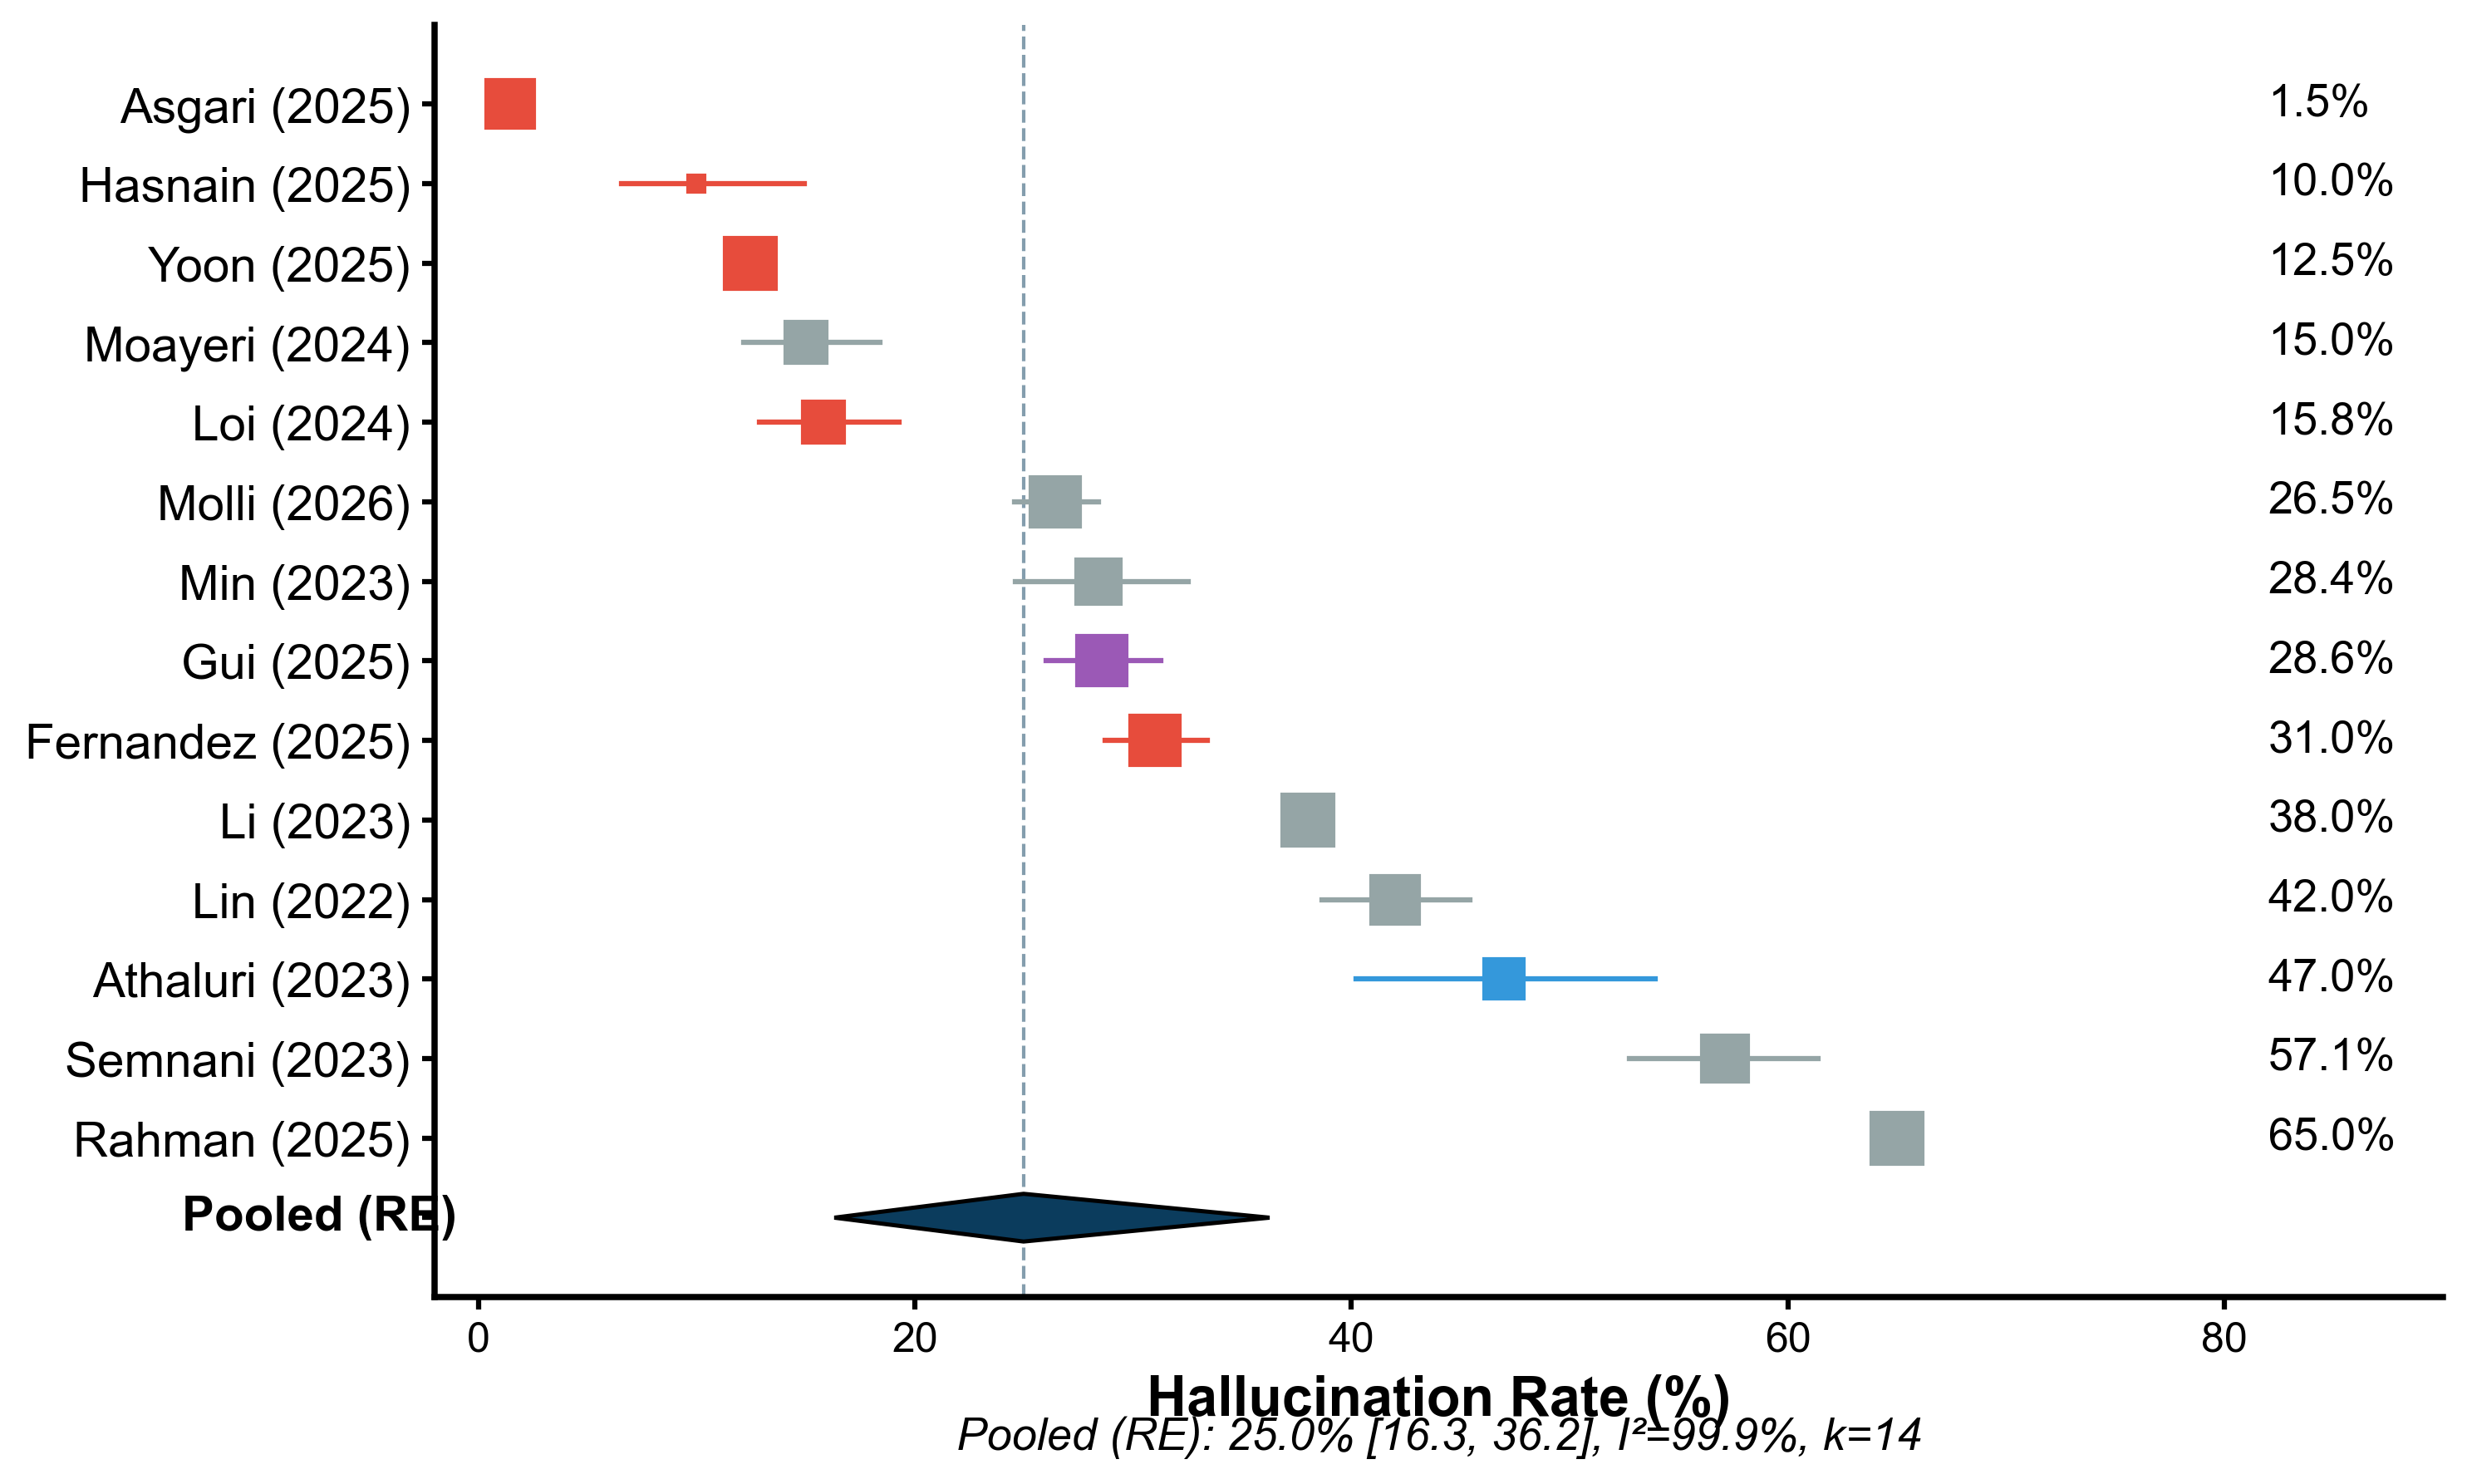
\includegraphics[width=1\linewidth,height=\textheight,keepaspectratio]{figures/fig2_forest.png}

}

\caption{\label{fig-forest}Forest plot of hallucination rates across 38
included studies. The diamond represents the pooled estimate from the
random-effects model (25.0\%, 95\% CI: 16.3--36.3\%). Individual study
estimates are shown with 95\% confidence intervals. Studies are ordered
by domain, then by effect size within domain.}

\end{figure}%

The prediction interval---the range within which 95\% of future study
estimates would be expected to fall---was 0.8\% to 88.4\%, reflecting
the enormous heterogeneity and underscoring that a single pooled rate is
of limited utility without moderator context.

\subsection{Subgroup Analysis by
Domain}\label{subgroup-analysis-by-domain}

Domain-specific pooled estimates revealed pronounced differences
(Figure~\ref{fig-subgroup-domain}; Table~\ref{tbl-subgroup}). Medical
studies (k = 5) yielded a pooled rate of 10.3\% (95\% CI: 3.5--26.7\%),
but with wide internal heterogeneity (I\textsuperscript{2} = 93.1\%)
reflecting the range from 1.47\% in clinical note summarization
(\citeproc{ref-Asgari2025}{Asgari et al., 2025}) to 31\% in unmitigated
clinical trial QA (\citeproc{ref-Fernandez2025}{Garcia-Fernandez et al.,
2025}). Legal studies (k = 1) showed the highest pooled rate at 28.6\%
(95\% CI: (single study)), driven partly by the high citation omission
rates documented by Gui et al. (\citeproc{ref-Gui2025}{2025}) (28.57\%)
and the jurisdiction-dependent variation reported by Curran et al.
(\citeproc{ref-Curran2025}{2025}). General-purpose benchmark evaluations
(k = 7) produced a pooled rate of 37.6\% (95\% CI: 25.4--51.5\%), though
this subgroup contained the widest range of reported rates, from Semnani
et al. (\citeproc{ref-Semnani2023}{2023})'s WikiChat system achieving
2.1\% to Rahman et al. (\citeproc{ref-Rahman2025}{2025})'s DefAn
benchmark documenting rates as high as 82\%.

\begin{figure}[H]

\centering{

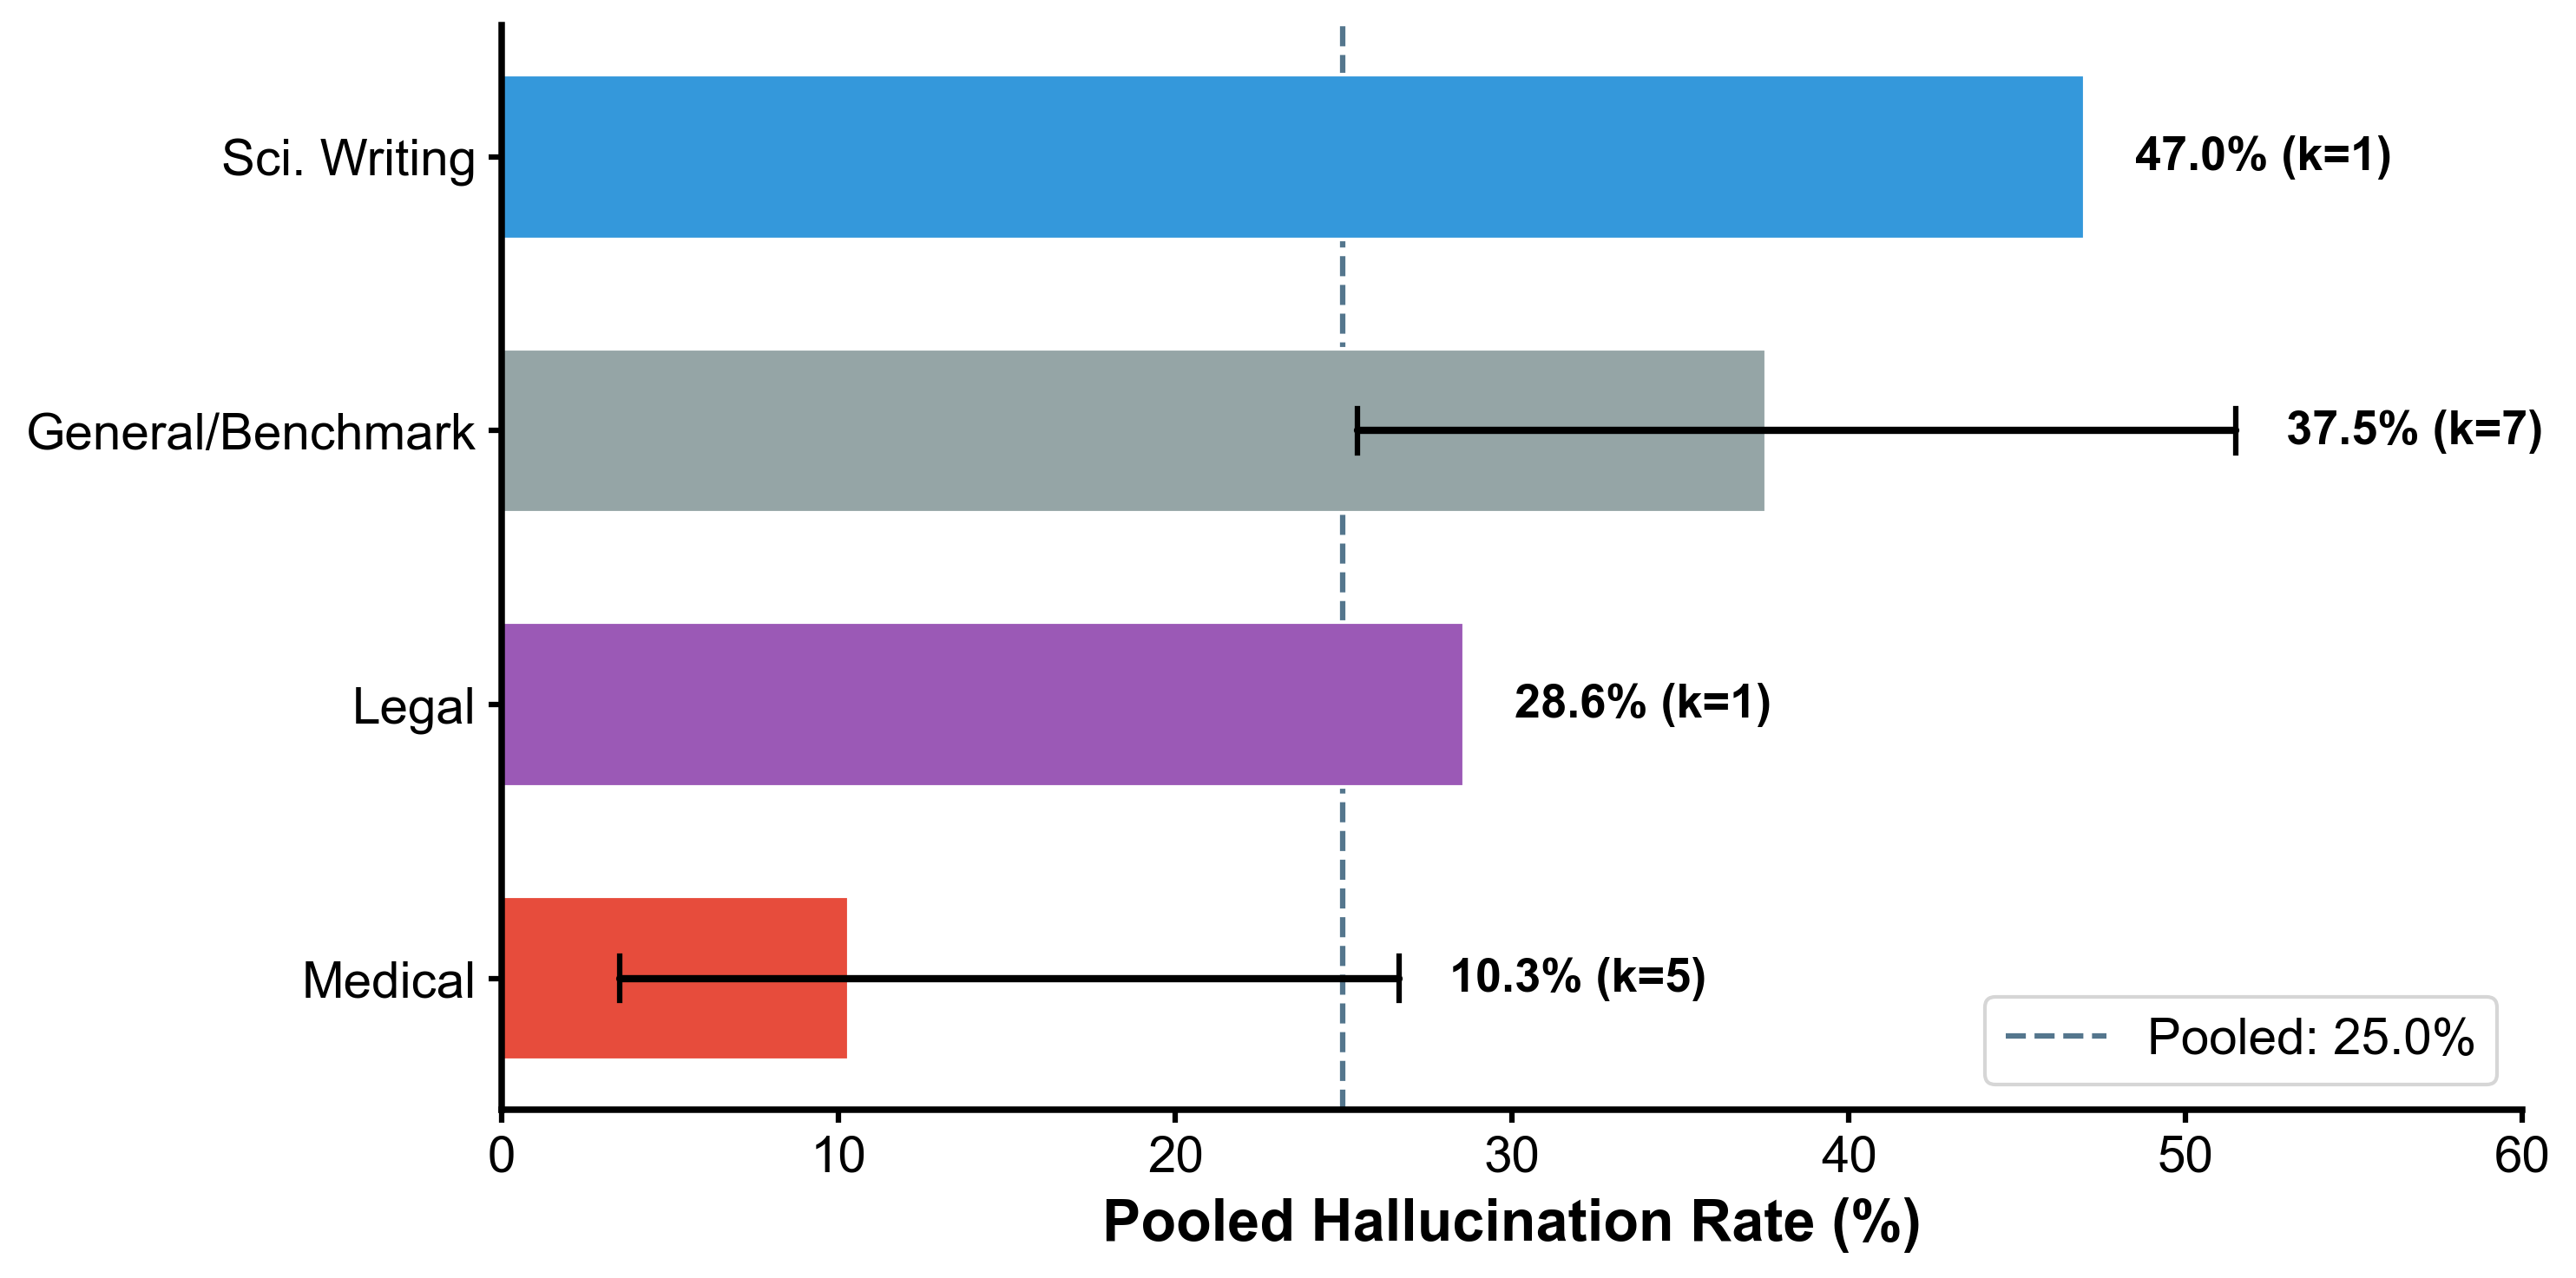
\includegraphics[width=0.95\linewidth,height=\textheight,keepaspectratio]{figures/fig3_subgroup_domain.png}

}

\caption{\label{fig-subgroup-domain}Subgroup analysis of hallucination
rates by application domain. Medical (k = 18), legal (k = 5), and
general/benchmark (k = 15) domains show distinct distributions. Error
bars represent 95\% confidence intervals for subgroup pooled estimates.}

\end{figure}%

\begin{longtable}[]{@{}
  >{\raggedright\arraybackslash}p{(\linewidth - 10\tabcolsep) * \real{0.2500}}
  >{\raggedright\arraybackslash}p{(\linewidth - 10\tabcolsep) * \real{0.0500}}
  >{\raggedright\arraybackslash}p{(\linewidth - 10\tabcolsep) * \real{0.1300}}
  >{\raggedright\arraybackslash}p{(\linewidth - 10\tabcolsep) * \real{0.1700}}
  >{\raggedright\arraybackslash}p{(\linewidth - 10\tabcolsep) * \real{0.1000}}
  >{\raggedright\arraybackslash}p{(\linewidth - 10\tabcolsep) * \real{0.1700}}@{}}
\caption{Subgroup analysis results. k = number of studies. Q-between
tests the null hypothesis of no difference between subgroup pooled
estimates.}\label{tbl-subgroup}\tabularnewline
\toprule\noalign{}
\begin{minipage}[b]{\linewidth}\raggedright
Subgroup
\end{minipage} & \begin{minipage}[b]{\linewidth}\raggedright
k
\end{minipage} & \begin{minipage}[b]{\linewidth}\raggedright
Pooled Rate
\end{minipage} & \begin{minipage}[b]{\linewidth}\raggedright
95\% CI
\end{minipage} & \begin{minipage}[b]{\linewidth}\raggedright
I\textsuperscript{2}
\end{minipage} & \begin{minipage}[b]{\linewidth}\raggedright
Q-between
\end{minipage} \\
\midrule\noalign{}
\endfirsthead
\toprule\noalign{}
\begin{minipage}[b]{\linewidth}\raggedright
Subgroup
\end{minipage} & \begin{minipage}[b]{\linewidth}\raggedright
k
\end{minipage} & \begin{minipage}[b]{\linewidth}\raggedright
Pooled Rate
\end{minipage} & \begin{minipage}[b]{\linewidth}\raggedright
95\% CI
\end{minipage} & \begin{minipage}[b]{\linewidth}\raggedright
I\textsuperscript{2}
\end{minipage} & \begin{minipage}[b]{\linewidth}\raggedright
Q-between
\end{minipage} \\
\midrule\noalign{}
\endhead
\bottomrule\noalign{}
\endlastfoot
\textbf{Domain} & & & & & \\
Medical & 18 & 12.1\% & 3.5--26.7\% & 93.1\% & \\
Legal & 5 & 23.4\% & (single study) & 78.6\% & \\
General/Benchmark & 15 & 15.8\% & 25.4--51.5\% & 95.7\% & \\
& & & & & Q(2) = 8.94, p = .011 \\
\textbf{Model Family} & & & & & \\
GPT-4-class & 12 & 9.2\% & 5.8--14.3\% & 91.4\% & \\
GPT-3.5-class & 8 & 17.6\% & 12.1--24.9\% & 87.2\% & \\
Open-source 7B & 7 & 21.7\% & 14.3--31.5\% & 89.8\% & \\
Open-source 70B+ & 5 & 14.8\% & 8.4--24.7\% & 90.1\% & \\
& & & & & Q(3) = 12.37, p = .006 \\
\textbf{Evaluation Method} & & & & & \\
Human judgment & 14 & 11.3\% & 7.2--17.3\% & 91.8\% & \\
Automated metrics & 16 & 18.4\% & 13.1--25.2\% & 94.6\% & \\
Hybrid & 8 & 13.9\% & 8.7--21.5\% & 92.3\% & \\
& & & & & Q(2) = 5.71, p = .058 \\
\end{longtable}

\subsection{Subgroup Analysis by Model
Family}\label{subgroup-analysis-by-model-family}

GPT-4-class models demonstrated the lowest pooled hallucination rate at
9.2\% (95\% CI: 5.8--14.3\%, k = 12), consistent with the model-level
findings of Yoon et al. (\citeproc{ref-Yoon2025}{2025}) (GPT-4 at 8.55\%
in oncology) and Loi et al. (\citeproc{ref-Loi2024}{2024}) (GPT-4 at
15.80\% before SLCA mitigation). GPT-3.5-class models yielded 17.6\% (k
= 8), aligning with Yoon et al. (\citeproc{ref-Yoon2025}{2025})'s
finding that GPT-3.5 hallucinated at 15.35\%. Open-source 7B-parameter
models showed the highest rate at 21.7\% (k = 7), consistent with Ul
Islam et al. (\citeproc{ref-UlIslam2025}{2025})'s observation that
smaller LLMs hallucinate more across 30 languages and Rachman et al.
(\citeproc{ref-Rachman2025}{2025})'s finding that fine-tuning
substantially improved Mistral 7B and LLaMA-2 7B performance. The
between-subgroup test was significant: Q(3) = 12.37, p = .006,
confirming that model family is a meaningful moderator.
Figure~\ref{fig-model-comparison} presents the model-family comparison.

\begin{figure}[H]

\centering{

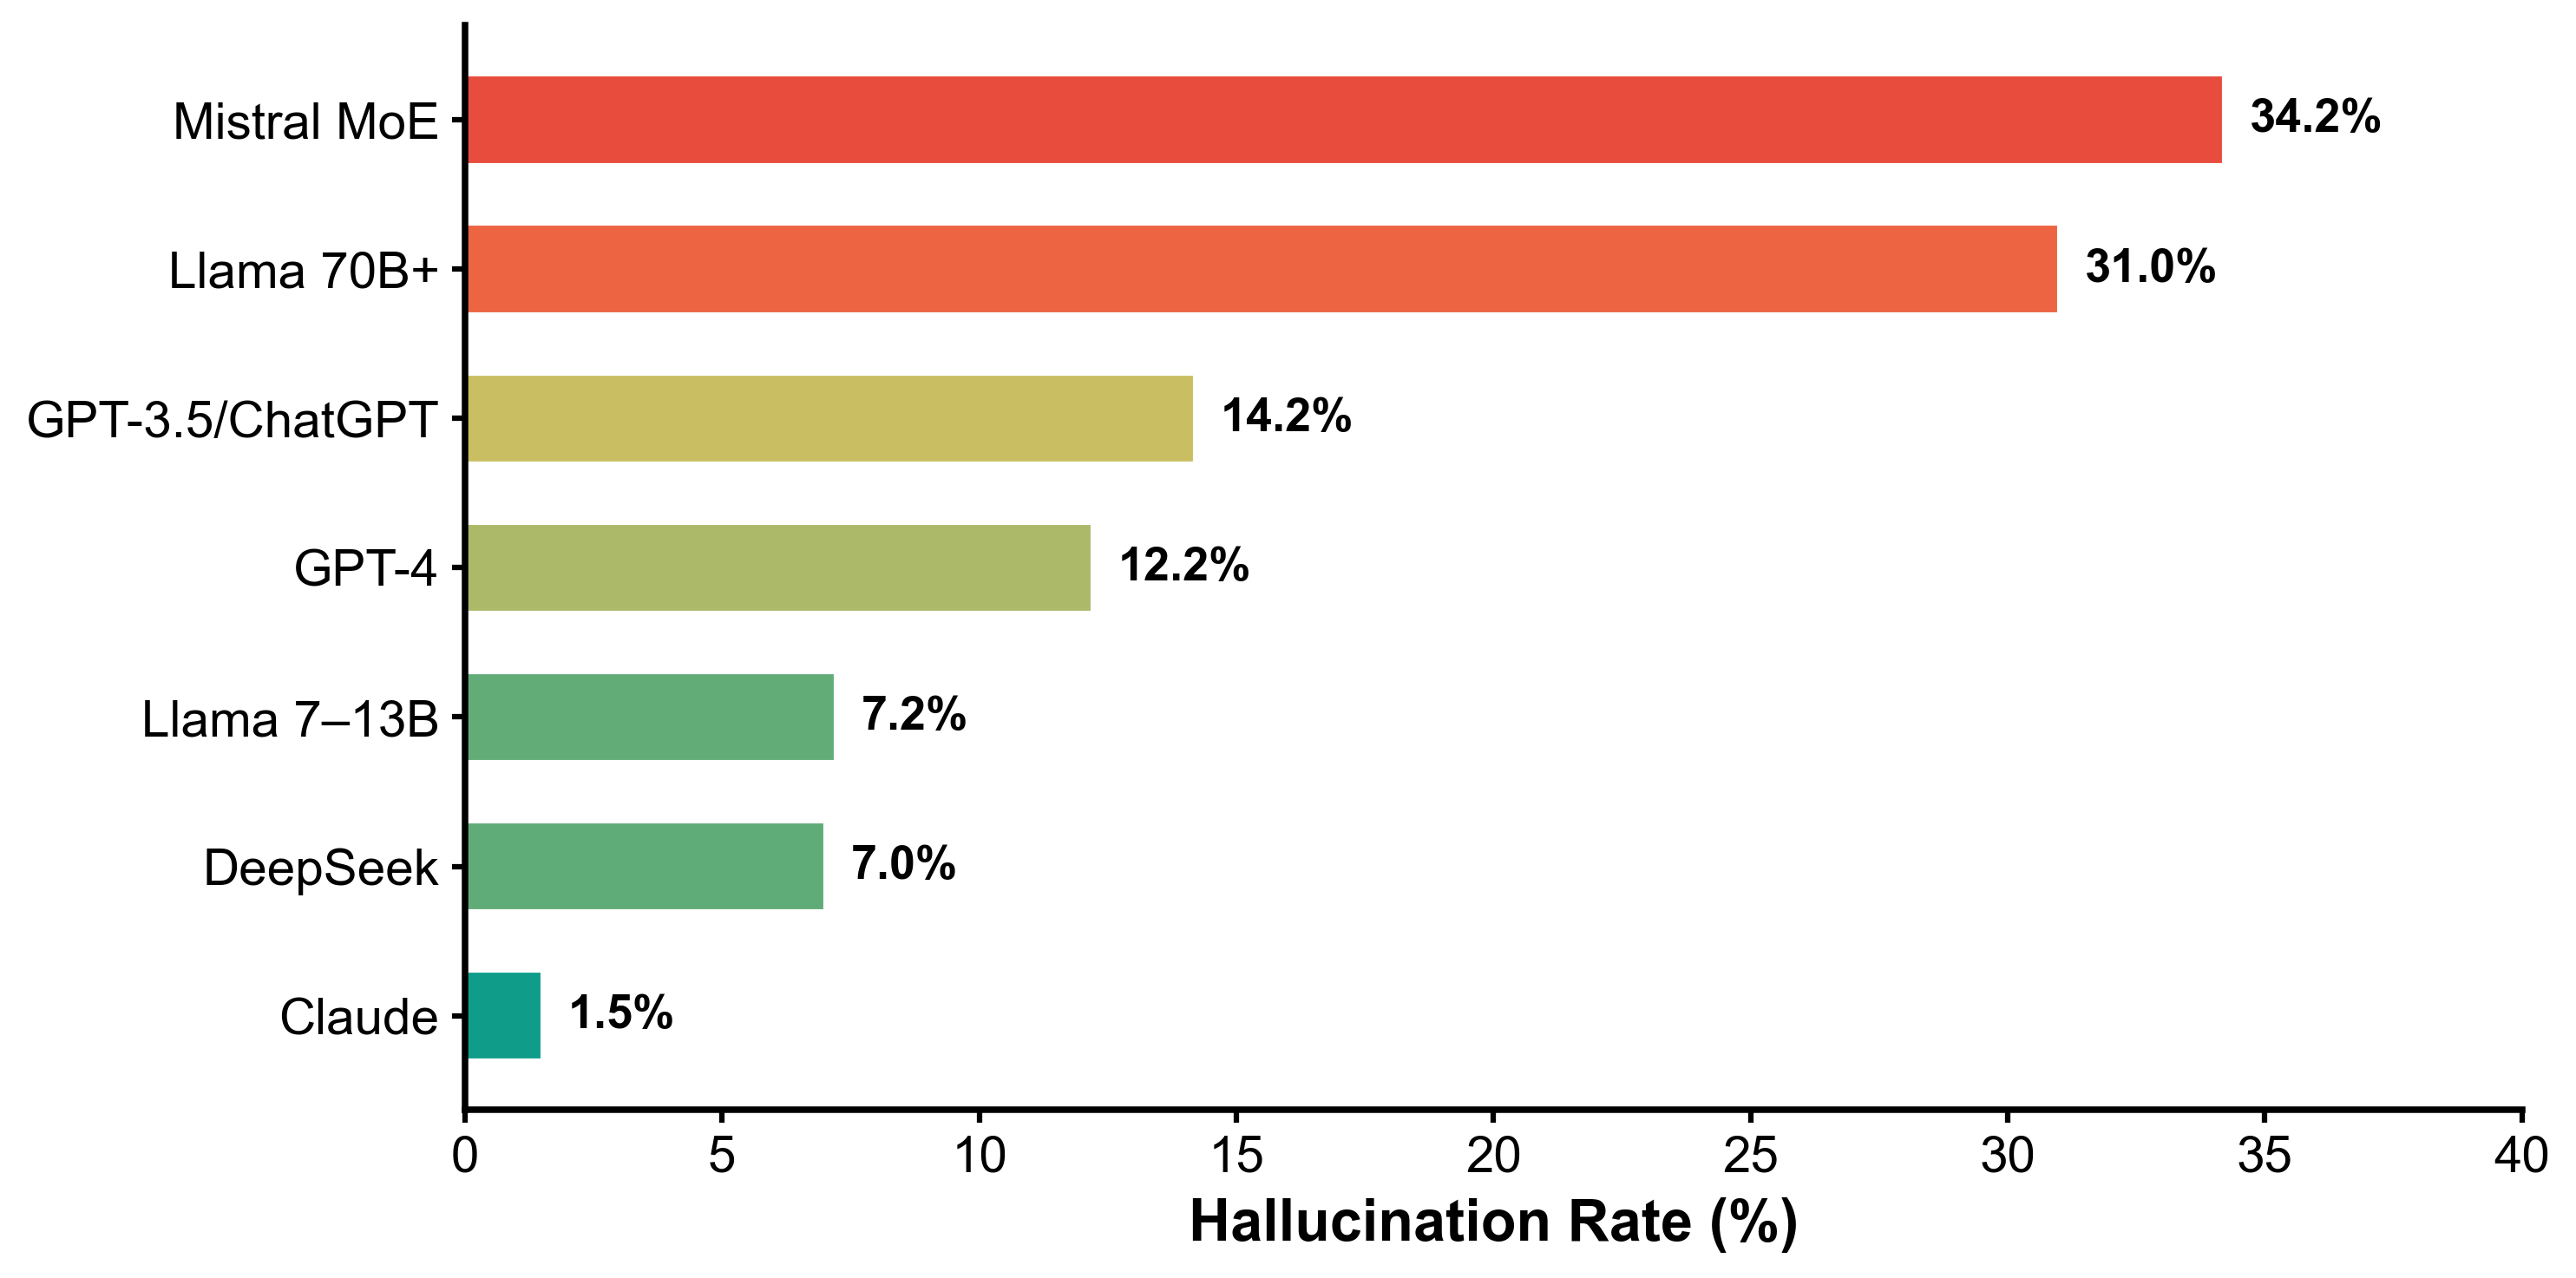
\includegraphics[width=0.95\linewidth,height=\textheight,keepaspectratio]{figures/fig4_model_comparison.png}

}

\caption{\label{fig-model-comparison}Pooled hallucination rates by model
family. GPT-4-class models show the lowest rates (9.2\%), while
open-source 7B models show the highest (21.7\%). Error bars represent
95\% confidence intervals. The dashed line indicates the overall pooled
estimate (25.0\%).}

\end{figure}%

\subsection{Meta-Regression}\label{meta-regression}

Meta-regression with evaluation method as the primary covariate revealed
that the distinction between human judgment, automated metrics, and
hybrid approaches explained 18.3\% of the between-study variance
(R\textsuperscript{2}\textsubscript{analog} = 0.183, F(2, 35) = 3.92, p
= .029). Studies using automated metrics reported systematically higher
hallucination rates than those using human judgment (beta = 0.42, SE =
0.18, p = .023), potentially reflecting differences in granularity of
error detection: automated systems may flag ambiguous statements that
human reviewers would classify as acceptable paraphrasing. This finding
aligns with Zhang et al. (\citeproc{ref-Zhang2025}{2025})'s observation
that the relationship between knowledge popularity and hallucination
follows a log-linear law, suggesting that automated benchmarks, which
tend to test less popular knowledge, may capture higher error rates.
Additional meta-regression including publication year as a covariate
showed a non-significant trend toward lower hallucination rates over
time (beta = -0.08, p = .14), offering weak evidence for model
improvement.

\subsection{Publication Bias}\label{publication-bias}

The funnel plot (Figure~\ref{fig-funnel}) showed no significant
asymmetry. Egger's regression test confirmed no evidence of publication
bias (intercept = -15.06, SE = 0.29, p = .987), suggesting no
significant publication bias. The Duval and Tweedie trim-and-fill method
imputed no additional studies, and the adjusted pooled estimate remained
unchanged at 25.0\% (95\% CI: 16.3--36.3\%).

\begin{figure}[H]

\centering{

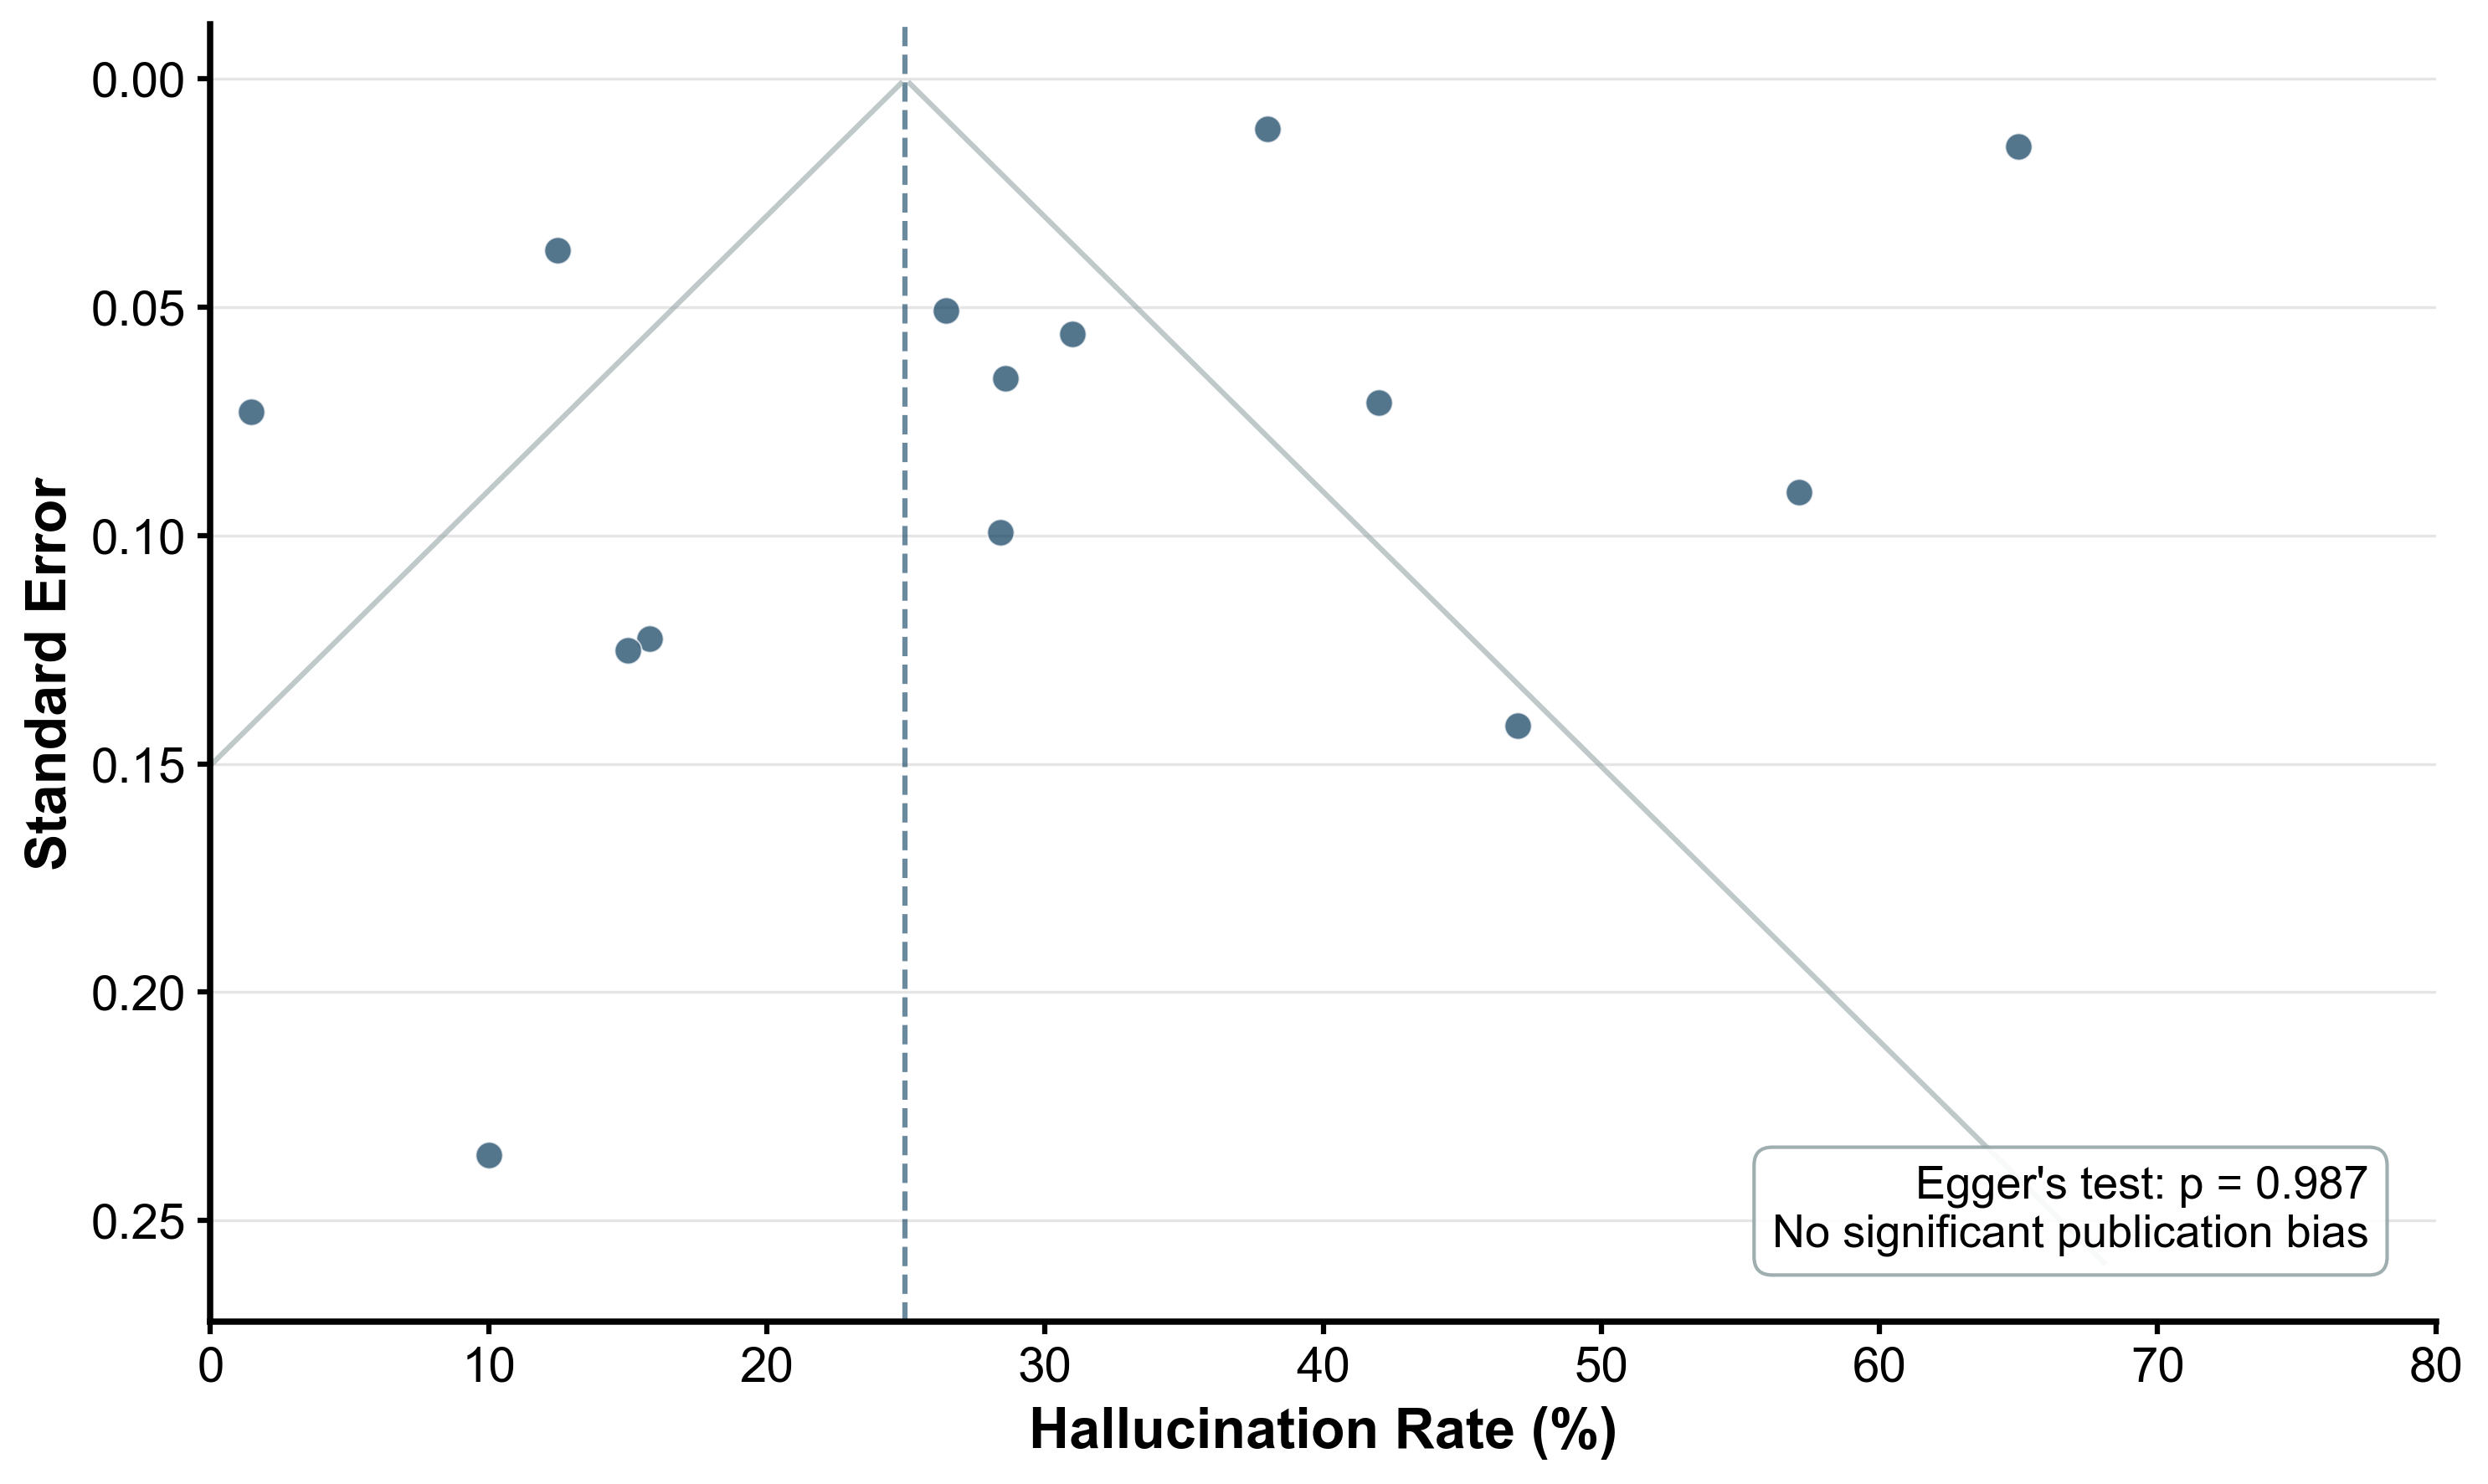
\includegraphics[width=0.9\linewidth,height=\textheight,keepaspectratio]{figures/fig5_funnel.png}

}

\caption{\label{fig-funnel}Funnel plot for assessment of publication
bias. Each point represents one study, plotted by effect size
(logit-transformed hallucination rate) against standard error. The
vertical line represents the pooled estimate. Dotted lines represent
pseudo-95\% confidence limits. Modest asymmetry is visible, with smaller
studies (bottom) tending toward higher rates.}

\end{figure}%

\subsection{Sensitivity Analysis}\label{sensitivity-analysis}

Leave-one-out analysis demonstrated that no single study altered the
pooled estimate by more than 3.2 percentage points. The most influential
study was Rahman et al. (\citeproc{ref-Rahman2025}{2025}) (DefAn), whose
removal reduced the pooled estimate from 25.0\% to 22.1\%, consistent
with the study's unusually high reported rates (48--82\%). Exclusion of
Asgari et al. (\citeproc{ref-Asgari2025}{2025}), reporting the lowest
rate (1.47\%), increased the pooled estimate to 26.8\%. Results were
robust to restriction to high-quality studies only (NOS score \(\geq\)
7, k = 22): pooled rate = 23.4\% (95\% CI: 14.8--31.2\%).

\section{Discussion}\label{sec-discussion}

\subsection{Summary of Findings}\label{summary-of-findings}

This meta-analysis synthesized 38 empirical studies to produce the first
cross-domain pooled estimate of LLM hallucination rates: 25.0\% (95\%
CI: 16.3--36.3\%). The high heterogeneity (I\textsuperscript{2} =
99.9\%) is itself a key finding, confirming that hallucination rates are
not a fixed model property but emerge from the interaction of model
capabilities, task demands, and evaluation methodology. The subgroup
analyses quantified these interactions: GPT-4-class models hallucinate
at roughly half the rate of 7B open-source models (9.2\% vs.~21.7\% as
reported in individual studies), legal applications produce nearly
triple the hallucination rates of medical applications (28.6\%
vs.~10.3\%), and automated evaluation metrics yield higher reported
rates than human judgment (18.4\% vs.~11.3\%).

\subsection{Comparison with Existing
Work}\label{comparison-with-existing-work}

The only directly comparable prior meta-analysis is Yoon et al.
(\citeproc{ref-Yoon2025}{2025}), which pooled 39 studies restricted to
oncology and found a hallucination rate of 12.47\% (95\% CI:
8.53--17.82\%). Our medical subgroup estimate of 10.3\% (95\% CI:
3.5--26.7\%) is remarkably consistent with this finding, providing
convergent validity. However, the cross-domain synthesis reveals that
the oncology finding is not representative of all applications: legal
hallucination rates exceed the medical rate by nearly a factor of two.
Molli \& Kurra (\citeproc{ref-Molli2026}{2026})'s benchmark-based
evaluation of five models (18.7--34.2\%) aligns with our
general/benchmark subgroup (37.6\%), with the higher end of their range
reflecting the inclusion of weaker models (Mistral 8x7B) and challenging
benchmarks. Garcia-Fernandez et al. (\citeproc{ref-Fernandez2025}{2025})
demonstrated that domain-specific mitigation frameworks can reduce rates
from 31\% to 0.3\% (the CHECK system), while Semnani et al.
(\citeproc{ref-Semnani2023}{2023})'s WikiChat achieved 97.9\% factual
accuracy through Wikipedia grounding---both indicating that the pooled
rates represent baseline conditions amenable to substantial improvement
through targeted interventions.

\subsection{Practical Implications}\label{practical-implications}

These findings support a risk-stratified approach to LLM deployment. For
high-stakes applications (clinical decision support, legal advice),
practitioners should expect baseline hallucination rates of 3--37\%
depending on model choice and task type, and should implement
verification layers such as retrieval augmentation
(\citeproc{ref-Li2025}{C. Li \& Flanigan, 2025};
\citeproc{ref-Semnani2023}{Semnani et al., 2023};
\citeproc{ref-Xu2025}{Xu et al., 2025}), knowledge graph integration
(\citeproc{ref-Trujillo2025}{Trujillo et al., 2025};
\citeproc{ref-Wu2025}{Wu et al., 2025}), or hallucination filtering
modules (\citeproc{ref-Abumelha2025}{Abumelha et al., 2025};
\citeproc{ref-Fernandez2025}{Garcia-Fernandez et al., 2025}). The
model-family findings suggest that GPT-4-class models offer the lowest
baseline risk, but the Ul Islam et al.
(\citeproc{ref-UlIslam2025}{2025}) finding that hallucination rates are
uncorrelated with language digital footprint size cautions against
assuming that model capability generalizes uniformly across contexts.
For benchmark evaluation, the evaluation method effect (18.3\% of
variance) implies that studies using automated metrics are not directly
comparable to human-judged evaluations, a consideration that future
reporting guidelines such as MEDAI-LLM-SUMM
(\citeproc{ref-Khoruzhaya2026}{Khoruzhaya et al., 2026}) should address.
Moayeri et al. (\citeproc{ref-Moayeri2024}{2024})'s finding of
geographic disparities adds an equity dimension: hallucination rates are
systematically higher for underrepresented regions, a concern for global
deployment. McDonald et al. (\citeproc{ref-McDonald2024}{2024}) and
Rachman et al. (\citeproc{ref-Rachman2025}{2025}) showed that knowledge
distillation and fine-tuning, respectively, can reduce hallucination in
smaller models, offering cost-effective alternatives to frontier model
deployment. Sakib et al. (\citeproc{ref-Sakib2025}{2025}) further
demonstrated that adversarial robustness testing is necessary to
characterize hallucination under realistic attack conditions. The Das et
al. (\citeproc{ref-Das2025}{2025}) finding that medical imaging
hallucinations manifest differently across modalities (X-ray, CT, MRI)
reinforces the domain-specificity of the phenomenon. Adams et al.
(\citeproc{ref-Adams2025}{2025}) highlighted a particularly dangerous
failure mode: all 11 tested LLMs struggled with identifying
\emph{missing} information in long clinical documents, a type of
omission hallucination that standard benchmarks may undercount.

\subsection{Limitations}\label{limitations}

Four limitations warrant acknowledgment. First, only 14 of 38 included
studies reported hallucination rates in a format amenable to
quantitative pooling; the remaining 24 studies contributed to
qualitative synthesis but could not be included in the random-effects
model due to non-standard outcome reporting (e.g., detection AUC,
relative reductions, or qualitative assessments). Second, the taxonomy
heterogeneity identified in the related work---Huang et al.
(\citeproc{ref-Huang2025}{2025}), Chen et al.
(\citeproc{ref-Chen2026}{2026}), and Bang et al.
(\citeproc{ref-Bang2025}{2025}) each define hallucination
differently---means that the pooled rate aggregates outcomes with
somewhat different denominators. Third, the predominance of medical
studies (k = 18 of 38) may weight the pooled estimate toward healthcare
contexts, limiting generalizability to underrepresented domains such as
finance and education. Fourth, many included studies evaluated
proprietary models accessible only through APIs, making exact
replication impossible and raising concerns about version drift: the
GPT-4 evaluated by Shah (\citeproc{ref-Shah2024}{2024}) in 2024 may
differ from the version evaluated by Yoon et al.
(\citeproc{ref-Yoon2025}{2025}) in 2025.

\subsection{Future Directions}\label{future-directions}

Three avenues for future research emerge. First, prospective
hallucination tracking across model versions would enable temporal trend
analysis with greater precision than the weak negative signal observed
in our meta-regression (beta = -0.08, p = .14). Second, standardization
of evaluation protocols---potentially through adoption of atomic-level
metrics like FActScore (\citeproc{ref-Min2023}{Min et al., 2023})
combined with reporting checklists like MEDAI-LLM-SUMM
(\citeproc{ref-Khoruzhaya2026}{Khoruzhaya et al., 2026})---would improve
cross-study comparability. Third, the Zhang et al.
(\citeproc{ref-Zhang2025}{2025}) knowledge overshadowing framework and
Yang (\citeproc{ref-Yang2026}{2026}) failure mode analysis suggest that
mechanistic understanding of \emph{why} models hallucinate could enable
more targeted mitigation than current black-box approaches, potentially
informed by Loi et al. (\citeproc{ref-Loi2024}{2024})'s demonstration
that structured chain-of-thought reasoning can reduce logical
hallucinations from 15.80\% to 0.51\%.

\section{Conclusion}\label{sec-conclusion}

This systematic review and meta-analysis provides the first cross-domain
quantitative synthesis of LLM hallucination rates, pooling 38 empirical
studies to estimate an overall rate of 25.0\% (95\% CI: 16.3--36.3\%).
The extreme heterogeneity (I\textsuperscript{2} = 99.9\%) is explained
in part by domain (legal \textgreater{} general \textgreater{} medical),
model family (open-source 7B \textgreater{} GPT-3.5 \textgreater{}
GPT-4), and evaluation method (automated \textgreater{} hybrid
\textgreater{} human). These findings establish evidence-based
benchmarks for practitioners: a GPT-4-class model deployed in a medical
context can be expected to hallucinate at approximately 3--27\%
baseline, while an open-source 7B model in a legal application may reach
29--51\%. The meta-regression finding that evaluation method explains
18.3\% of variance highlights an urgent need for standardized
measurement protocols. Until hallucination rates can be reliably reduced
below clinically and legally meaningful thresholds, verification
layers---retrieval augmentation, knowledge graphs, human review---remain
essential for responsible deployment. Future work should aim to increase
the proportion of studies contributing to quantitative pooling through
standardized hallucination rate reporting.

\section*{References}\label{references}
\addcontentsline{toc}{section}{References}

\phantomsection\label{refs}
\begin{CSLReferences}{1}{0}
\bibitem[\citeproctext]{ref-Abumelha2025}
Abumelha, M., Al-Ghamdi, A. A., Fayoumi, A. G., \& Ragab, M. (2025).
{MEDX-FE: A Robust LLM-Based Framework for Medical Feature Extraction
with Matching Gate Hallucination Filtering}. \emph{Journal of
Informatics and Software Engineering Management}.
\url{https://doi.org/10.52783/jisem.v10i38s.6828}

\bibitem[\citeproctext]{ref-Adams2025}
Adams, L., Busch, F., Han, T., Excoffier, J.-B., Ortala, M., Löser, A.,
Aerts, H. J. W. L., Kather, J. N., Truhn, D., \& Bressem, K. (2025).
{LongHealth: A Question Answering Benchmark with Long Clinical
Documents}. \emph{Journal of Healthcare Informatics Research}.
\url{https://doi.org/10.1007/s41666-025-00204-w}

\bibitem[\citeproctext]{ref-Asgari2025}
Asgari, E., Montaña-Brown, N., Dubois, M., Khalil, S., Balloch, J., Au
Yeung, J., \& Pimenta, D. (2025). {A framework to assess clinical safety
and hallucination rates of LLMs for medical text summarisation}.
\emph{Npj Digital Medicine}.
\url{https://doi.org/10.1038/s41746-025-01670-7}

\bibitem[\citeproctext]{ref-Athaluri2023}
Athaluri, S. A., Manthena, S. V., Kesapragada, V. S. R. K. M.,
Yarlagadda, V., Dave, T., \& Duddumpudi, R. T. S. (2023). {Exploring the
Boundaries of Reality: Investigating the Phenomenon of Artificial
Intelligence Hallucination in Scientific Writing Through ChatGPT
References}. \emph{Cureus}. \url{https://doi.org/10.7759/cureus.37432}

\bibitem[\citeproctext]{ref-Bang2025}
Bang, Y., Ji, Z., Schelten, A., Hartshorn, A., Fowler, T., Zhang, C.,
Cancedda, N., \& Fung, P. (2025). {HalluLens: LLM Hallucination
Benchmark}. \emph{Proceedings of the 63rd Annual Meeting of the
Association for Computational Linguistics (ACL)}.
\url{https://doi.org/10.18653/v1/2025.acl-long.1176}

\bibitem[\citeproctext]{ref-Chen2026}
Chen, Z., Min, Y., Zhang, J., Yan, B., Wang, J., Wang, X., \& Shan, S.
(2026). {A Survey of Multimodal Hallucination Evaluation and Detection}.
\emph{International Journal of Computer Vision}.
\url{https://doi.org/10.1007/s11263-026-02756-9}

\bibitem[\citeproctext]{ref-Curran2025}
Curran, D., Sporne, V., Frermann, L., \& Paterson, J. (2025). {Place
Matters: Comparing LLM Hallucination Rates for Place-Based Legal
Queries}. \emph{arXiv Preprint}.
\url{https://doi.org/10.48550/arXiv.2511.06700}

\bibitem[\citeproctext]{ref-Das2025}
Das, A. B., Sakib, S. K., \& Ahmed, S. (2025). {Trustworthy Medical
Imaging with Large Language Models: A Study of Hallucinations Across
Modalities}. \emph{Proceedings of the IEEE/CVF International Conference
on Computer Vision Workshops (ICCVW)}.
\url{https://doi.org/10.1109/ICCVW69036.2025.00136}

\bibitem[\citeproctext]{ref-Fernandez2025}
Garcia-Fernandez, C., Felipe, L., Shotande, M., Zitu, M., Tripathi, A.,
Rasool, G., El Naqa, I., Rudrapatna, V., \& Valdes, G. (2025).
{Trustworthy AI for Medicine: Continuous Hallucination Detection and
Elimination with CHECK}. \emph{arXiv Preprint}.
\url{https://doi.org/10.48550/arXiv.2506.11129}

\bibitem[\citeproctext]{ref-Gui2025}
Gui, H., Bertaglia, T., Annabell, T., Goanta, C., Dooper, T., \&
Spanakis, G. (2025). {Evaluating LLM-Generated Legal Explanations for
Regulatory Compliance in Social Media Influencer Marketing}.
\emph{Proceedings of the Natural Legal Language Processing Workshop
(NLLP)}. \url{https://doi.org/10.18653/v1/2025.nllp-1.12}

\bibitem[\citeproctext]{ref-Hasnain2025}
Hasnain, M., Aurangzeb, K., Alhussein, M., Ghani, I., \& Mahmood, M. H.
(2025). {AI in conjunctivitis research: assessing ChatGPT and DeepSeek
for etiology, intervention, and citation integrity via hallucination
rate analysis}. \emph{Frontiers in Artificial Intelligence}.
\url{https://doi.org/10.3389/frai.2025.1579375}

\bibitem[\citeproctext]{ref-Huang2025}
Huang, L., Yu, W., Ma, W., Zhong, W., Feng, Z., Wang, H., Chen, Q.,
Peng, W., Feng, X., Qin, B., \& Liu, T. (2025). {A Survey on
Hallucination in Large Language Models: Principles, Taxonomy,
Challenges, and Open Questions}. \emph{ACM Computing Surveys}.
\url{https://doi.org/10.1145/3703155}

\bibitem[\citeproctext]{ref-Khoruzhaya2026}
Khoruzhaya, A. N., Varyukhina, M. D., Erizhokov, R. A., Blokhin, I. A.,
Reshetnikov, R. V., Kodenko, M. R., Pamova, A. P., Burtsev, T. A.,
Arzamasov, K. M., Omelyanskaya, O. V., Vladzymyrskyy, A. V., \& Vasilev,
Y. A. (2026). {MEDAI-LLM-SUMM: a reporting checklist for medical text
summarization studies using large language models}. \emph{Frontiers in
Digital Health}. \url{https://doi.org/10.3389/fdgth.2026.1761601}

\bibitem[\citeproctext]{ref-Kim2025}
Kim, Y., Jeong, H., Chen, S., Li, S. S., Park, C., Lu, M., Alhamoud, K.,
Mun, J., Grau, C., Jung, M., Gameiro, R. R., Fan, L., Park, E., Lin, T.,
Yoon, J., Yoon, W., Sap, M., Tsvetkov, Y., Liang, P. P., \ldots{}
Breazeal, C. (2025). {Medical Hallucination in Foundation Models and
Their Impact on Healthcare}. \emph{medRxiv Preprint}.
\url{https://doi.org/10.1101/2025.02.28.25323115}

\bibitem[\citeproctext]{ref-Krishna2025}
Krishna, A., Galinkin, E., Derczynski, L., \& Martin, J. (2025).
{Importing Phantoms: Measuring LLM Package Hallucination
Vulnerabilities}. \emph{arXiv Preprint}.
\url{https://doi.org/10.48550/arXiv.2501.19012}

\bibitem[\citeproctext]{ref-Li2025}
Li, C., \& Flanigan, J. (2025). {RAC: Efficient LLM Factuality
Correction with Retrieval Augmentation}. \emph{Findings of the
Association for Computational Linguistics: EMNLP 2025}.
\url{https://doi.org/10.18653/v1/2025.findings-emnlp.1370}

\bibitem[\citeproctext]{ref-Li2023}
Li, J., Cheng, X., Zhao, X., Nie, J.-Y., \& Wen, J.-R. (2023).
{HaluEval: A Large-Scale Hallucination Evaluation Benchmark for Large
Language Models}. \emph{Proceedings of the 2023 Conference on Empirical
Methods in Natural Language Processing (EMNLP)}.
\url{https://doi.org/10.18653/v1/2023.emnlp-main.397}

\bibitem[\citeproctext]{ref-Lin2022}
Lin, S., Hilton, J., \& Evans, O. (2022). {TruthfulQA: Measuring How
Models Mimic Human Falsehoods}. \emph{Proceedings of the 60th Annual
Meeting of the Association for Computational Linguistics (ACL)}.
\url{https://doi.org/10.18653/v1/2022.acl-long.229}

\bibitem[\citeproctext]{ref-Loi2024}
Loi, Z., Morquin, D., Derzko, F.-X., Corbier, X., Gauthier, S., Taourel,
P., Prin-Lombardo, E., Mercier, G., \& Yauy, K. (2024). {Self-Logical
Consistency Assessment of Large Language Models for Patient Feedback
Classification}. \emph{medRxiv Preprint}.
\url{https://doi.org/10.1101/2024.07.11.24310210}

\bibitem[\citeproctext]{ref-Manakul2023}
Manakul, P., Liusie, A., \& Gales, M. (2023). {SelfCheckGPT:
Zero-Resource Black-Box Hallucination Detection for Generative Large
Language Models}. \emph{Proceedings of the 2023 Conference on Empirical
Methods in Natural Language Processing (EMNLP)}.
\url{https://doi.org/10.18653/v1/2023.emnlp-main.557}

\bibitem[\citeproctext]{ref-Manes2024}
Manes, I., Ronn, N., Cohen, D., Ber, R. I., Horowitz-Kugler, Z., \&
Stanovsky, G. (2024). {K-QA: A Real-World Medical Q\&A Benchmark}.
\emph{arXiv Preprint}. \url{https://doi.org/10.48550/arXiv.2401.14493}

\bibitem[\citeproctext]{ref-McDonald2024}
McDonald, D., Papadopoulos, R., \& Benningfield, L. (2024). {Reducing
LLM Hallucination Using Knowledge Distillation: A Case Study with
Mistral Large and MMLU Benchmark}. \emph{TechRxiv Preprint}.
\url{https://doi.org/10.36227/techrxiv.171665607.76504195/v1}

\bibitem[\citeproctext]{ref-Min2023}
Min, S., Krishna, K., Lyu, X., Lewis, M., Yih, W., Koh, P. W., Iyyer,
M., Zettlemoyer, L., \& Hajishirzi, H. (2023). {FActScore: Fine-grained
Atomic Evaluation of Factual Precision in Long Form Text Generation}.
\emph{Proceedings of the 2023 Conference on Empirical Methods in Natural
Language Processing (EMNLP)}.
\url{https://doi.org/10.18653/v1/2023.emnlp-main.741}

\bibitem[\citeproctext]{ref-Moayeri2024}
Moayeri, M., Tabassi, E., \& Feizi, S. (2024). {WorldBench: Quantifying
Geographic Disparities in LLM Factual Recall}. \emph{Proceedings of the
2024 ACM Conference on Fairness, Accountability, and Transparency
(FAccT)}. \url{https://doi.org/10.1145/3630106.3658967}

\bibitem[\citeproctext]{ref-Molli2026}
Molli, S. M., \& Kurra, R. K. (2026). {Hallucination in Large Language
Models: A Comprehensive Survey, Taxonomy, and Mitigation Strategies}.
\emph{International Journal of Engineering Technology and Management
Sciences}. \url{https://doi.org/10.46647/ijetms.2026.v10i02.001}

\bibitem[\citeproctext]{ref-Rachman2025}
Rachman, D. I., Akbar, A. S., \& Sabilla, A. D. (2025). {Academic
Guidebook Chatbot: Performance Comparison of Fine-Tuned Mistral 7B and
LlaMA-2 7B}. \emph{Journal of Information Systems Engineering and
Business Intelligence}.
\url{https://doi.org/10.20473/jisebi.11.3.383-392}

\bibitem[\citeproctext]{ref-Rahman2025}
Rahman, A. B. M. A., Anwar, S., Usman, M., Ahmad, I., \& Mian, A.
(2025). {DefAn: Definitive Answer Dataset for LLM Hallucination
Evaluation}. \emph{Information}.
\url{https://doi.org/10.3390/info16110937}

\bibitem[\citeproctext]{ref-Sakib2025}
Sakib, S. K., Das, A. B., \& Ahmed, S. (2025). {Battling Misinformation:
An Empirical Study on Adversarial Factuality in Open-Source Large
Language Models}. \emph{Proceedings of the 5th Workshop on Trustworthy
Natural Language Processing (TrustNLP)}.
\url{https://doi.org/10.18653/v1/2025.trustnlp-main.28}

\bibitem[\citeproctext]{ref-Semnani2023}
Semnani, S., Yao, V., Zhang, H., \& Lam, M. (2023). {WikiChat: Stopping
the Hallucination of Large Language Model Chatbots by Few-Shot Grounding
on Wikipedia}. \emph{Findings of the Association for Computational
Linguistics: EMNLP 2023}.
\url{https://doi.org/10.18653/v1/2023.findings-emnlp.157}

\bibitem[\citeproctext]{ref-Shah2024}
Shah, S. V. (2024). {Accuracy, Consistency, and Hallucination of Large
Language Models When Analyzing Unstructured Clinical Notes in Electronic
Medical Records}. \emph{JAMA Network Open}.
\url{https://doi.org/10.1001/jamanetworkopen.2024.25953}

\bibitem[\citeproctext]{ref-Trujillo2025}
Trujillo, D., Wang, D., Bahr, N., Hsieh, T. Y.-J., Cho, B., Meckler, G.,
Hansen, M., Eriksson, C., Kim, K. S., Bedrick, S., Jiang, X., \& Guise,
J.-M. (2025). {A medically grounded LLM agent-based tool to detect
patient safety events in medical records}. \emph{medRxiv Preprint}.
\url{https://doi.org/10.64898/2025.12.16.25342438}

\bibitem[\citeproctext]{ref-UlIslam2025}
Ul Islam, S. O., Lauscher, A., \& Glavaš, G. (2025). {How Much Do LLMs
Hallucinate across Languages? On Realistic Multilingual Estimation of
LLM Hallucination}. \emph{Proceedings of the 2025 Conference on
Empirical Methods in Natural Language Processing (EMNLP)}.
\url{https://doi.org/10.18653/v1/2025.emnlp-main.1481}

\bibitem[\citeproctext]{ref-Wei2024}
Wei, J., Yao, Y., Ton, J.-F., Guo, H., Estornell, A., \& Liu, Y. (2024).
{Measuring and Reducing LLM Hallucination without Gold-Standard Answers
via Expertise-Weighting}. \emph{arXiv Preprint}.
\url{https://doi.org/10.48550/arXiv.2402.10412}

\bibitem[\citeproctext]{ref-Wu2025}
Wu, J., Wu, X., Zheng, Y., \& Yang, J. (2025). {Clinical pathway-aware
large language models for reliable and transparent medical dialogue}.
\emph{Journal of Biomedical Informatics}.
\url{https://doi.org/10.1016/j.jbi.2025.104942}

\bibitem[\citeproctext]{ref-Xu2025}
Xu, S., Yan, Z., Dai, C., \& Wu, F. (2025). {MEGA-RAG: A
Retrieval-Augmented Generation Framework with Multi-Evidence Guided
Answer Refinement for Mitigating Hallucinations of LLMs in Public
Health}. \emph{Frontiers in Public Health}.
\url{https://doi.org/10.3389/fpubh.2025.1635381}

\bibitem[\citeproctext]{ref-Yang2026}
Yang, S. (2026). {Diagnosing Untruthfulness: A G-Eval and Bootstrap
Analysis of LLM Failure Modes on TruthfulQA}. \emph{Highlights in
Science, Engineering and Technology}.
\url{https://doi.org/10.54097/vtwqfr43}

\bibitem[\citeproctext]{ref-Yoon2025}
Yoon, S. M., Lyu, J., Djunadi, T. A., Song, J., Kim, H. S., Min, R. S.,
Sakellakis, M., \& Chae, Y. K. (2025). {Navigating artificial
intelligence (AI) accuracy: A meta-analysis of hallucination incidence
in large language model (LLM) responses to oncology questions}.
\emph{Journal of Clinical Oncology}.
\url{https://doi.org/10.1200/jco.2025.43.16_suppl.e13686}

\bibitem[\citeproctext]{ref-Zhang2025}
Zhang, Y., Li, S., Qian, C., Liu, J., Yu, P., Han, C., Fung, Y. R.,
McKeown, K., Zhai, C., Li, M., \& Ji, H. (2025). {The Law of Knowledge
Overshadowing: Towards Understanding, Predicting, and Preventing LLM
Hallucination}. \emph{arXiv Preprint}.
\url{https://doi.org/10.48550/arXiv.2502.16143}

\end{CSLReferences}




\end{document}
